% multiple1902 <multiple1902@gmail.com>
% master.tex
% Copyright 2011~2012, multiple1902 (Weisi Dai)
% https://code.google.com/p/xjtuthesis/
%
% It is strongly recommended that you read documentations located at
%   http://code.google.com/p/xjtuthesis/wiki/Landing?tm=6
% in advance of your compilation if you have not read them before.
%
% This work may be distributed and/or modified under the
% conditions of the LaTeX Project Public License, either version 1.3
% of this license or (at your option) any later version.
% The latest version of this license is in
%   http://www.latex-project.org/lppl.txt
% and version 1.3 or later is part of all distributions of LaTeX
% version 2005/12/01 or later.
%
% This work has the LPPL maintenance status `maintained'.
%
% The Current Maintainer of this work is Weisi Dai.
%
\documentclass[
    master,
    truefont, % just turn it on when using Windows
    %nofont, % remember to manally set the fonts
    pdflinks,
    %colorlinks,
    % compact,
    ]{xjtuthesis}

\usepackage{threeparttable}
\usepackage{tabularx}
\usepackage{tikz}
\usepackage{listings}

\definecolor{dkgreen}{rgb}{0,0.6,0}
\definecolor{gray}{rgb}{0.5,0.5,0.5}
\definecolor{mauve}{rgb}{0.58,0,0.82}

\lstset{ %
  language=Octave,                % the language of the code
  basicstyle=\small,           % the size of the fonts that are used for the code
  %numbers=left,                   % where to put the line-numbers
  numberstyle=\tiny\color{gray},  % the style that is used for the line-numbers
  stepnumber=2,                   % the step between two line-numbers. If it's 1, each line
                                  % will be numbered
  numbersep=5pt,                  % how far the line-numbers are from the code
  backgroundcolor=\color{white},      % choose the background color. You must add \usepackage{color}
  showspaces=false,               % show spaces adding particular underscores
  showstringspaces=false,         % underline spaces within strings
  showtabs=false,                 % show tabs within strings adding particular underscores
  frame=single,                   % adds a frame around the code
  rulecolor=\color{black},        % if not set, the frame-color may be changed on line-breaks within not-black text (e.g. commens (green here))
  tabsize=2,                      % sets default tabsize to 2 spaces
  captionpos=b,                   % sets the caption-position to bottom
  breaklines=true,                % sets automatic line breaking
  breakatwhitespace=false,        % sets if automatic breaks should only happen at whitespace
  title=\lstname,                   % show the filename of files included with \lstinputlisting;
                                  % also try caption instead of title
  keywordstyle=\color{blue},          % keyword style
  commentstyle=\color{dkgreen},       % comment style
  stringstyle=\color{mauve},         % string literal style
  escapeinside={\%*}{*)},            % if you want to add LaTeX within your code
  morekeywords={*,...}               % if you want to add more keywords to the set
}

\usetikzlibrary{shapes.geometric, arrows}

\hyphenation{op-tical net-works semi-conduc-tor}

\graphicspath{{figures/}}

\begin{document}

    % 请修改 meta.tex 中的论文元信息
    % multiple1902 <multiple1902@gmail.com>
% meta.tex
% Copyright 2011~2012, multiple1902 (Weisi Dai)
% https://code.google.com/p/xjtuthesis/
%
% It is strongly recommended that you read documentations located at
%   http://code.google.com/p/xjtuthesis/wiki/Landing?tm=6
% in advance of your compilation if you have not read them before.
%
% This work may be distributed and/or modified under the
% conditions of the LaTeX Project Public License, either version 1.3
% of this license or (at your option) any later version.
% The latest version of this license is in
%   http://www.latex-project.org/lppl.txt
% and version 1.3 or later is part of all distributions of LaTeX
% version 2005/12/01 or later.
%
% This work has the LPPL maintenance status `maintained'.
%
% The Current Maintainer of this work is Weisi Dai.
%

% 标题,中文
\ctitle{连铸坯表面缺陷检测方法研究}

% 作者,中文
\cauthor{ }

% 学科,中文,本科生不需要
\csubject{软件工程}

% 导师姓名,中文
\csupervisor{ }

% 关键词,中文。用全角分号「;」分割
% 研究生的应首先从《汉语主题词表》中摘选
\ckeywords{缺陷检测;显著性检测;深度图像;基准面;图像分割;法向量}

% 提交日期,本科生不需要
\cproddate{\the\year 年\the\month 月}

% 论文类型,中文,本科生不需要
% 从理论研究、应用基础、应用研究、研究报告、软件开发、设计报告、案例分析、调研报告、其它中选择
\ctype{应用研究}

% 论文标题,英文
\etitle{Research of suface defect detection method for continuous casting slab}

% 作者姓名,英文
\eauthor{ }

% 学科,英文,本科生不需要
\esubject{Software Engineering}

% 导师姓名,英文
\esupervisor{ }

% 关键词,英文。用半角分号和一个半角空格「; 」分割
\ekeywords{defect detection; saliency detection; depth map; datum plane; image segmentation; normal vector}

% 学科门类,英文
% 从Philosophy(哲学)、Economics(经济学)、Law(法学)、Education(教育学)、Arts(文学)、
%   Science(理学)、Engineering Science(工学)、Medicine(医学)、Management Science(管理学)中选择
\ecate{Engineering Science}

% 提交日期,英文,本科生不需要
% 应当和 cproddate 保持一致
\eproddate{\monthname{\month}\ \the\year}

% 论文类型,英文,本科生不需要
% 从Theoretical Research(理论研究)、Application Fundamentals(应用基础)、Applied Research(应用研究)、
%   Research Report(研究报告)、Software Development(软件开发)、Design Report(设计报告)、
%   Case Study(案例分析)、Investigation Report(调研报告)、其它(Other)中选择
\etype{Applied Research}

% 摘要,中文。段间空行
\cabstract{
自连铸机诞生以来,高温状态下钢板实时缺陷检测一直是热门的研究领域,实现这一技术可以避免存在缺陷的半成品钢材无意义的继续加工,提高热送率,增加生产效率。钢板表面的缺陷检测往往充满挑战,主要因为钢板表面的情况复杂、光照不均、存在氧化铁皮这种伪缺陷等等。

为了解决连铸坯表面黑斑的干扰,本文首先提出了一种基于显著性的钢板表面缺陷检测方法,该方法引入视觉显著性原理通过提升图像缺陷区域与背景区域的对比度来提高缺陷查全率,同时通过在多个尺度上应用视觉显著性特征来去除黑斑对检测结果的干扰,从而有效地降低缺陷的误检率,最后通过实验证明,该方法具有很好的检测效果,并且实时性高,符合工业生产的需要。然而,该方法只能专门去除黑斑这种伪缺陷,对于其他的伪缺陷检测效果不佳。

基于RGB图像的方法往往难以将伪缺陷和真正的缺陷区分开来,因此,本文提出了两种基于深度图像的钢板表面缺陷检测算法,分别是基于基准面的缺陷检测算法和基于法向量的缺陷检测算法,它们主要利用深度信息来检测钢板表面缺陷,能够有效地应对上述这些难点。基于基准面的缺陷检测算法希望能找到深度图像的基准面,然后将深度值与基准面差别较大的缺陷区域提取并分割出来。

基于基准面拟合的方法非常依赖于基准面拟合的准确,并且该方法查准率较低,为了解决上述问题,提出了基于法向量的方法。基于法向量的缺陷检测算法使用法向量梯度图像来刻画法向量的变化程度,然后根据法向量梯度图像将缺陷区域分割出来。

最后,为了验证本文提出的基于深度图像的缺陷检测算法,基于真实的钢板深度数据,本文使用人工合成手段构建了一个钢板深度图像数据集。在该数据集上的实验结果显示,本文提出的两个缺陷检测算法都达到了很好的效果,能够有效地检测出钢板表面缺陷。
}

% 摘要,英文。段间空行
\eabstract{
Real-time defect detection for high temperature steel slabs is always one of the hot research fields since continuous casting machine appeared. Realizing the technique would avoid unnecessary processing of the defective semi-finished product, raise hot delivery rate and increase production efficiency. Defect detection on steel surface is challenging owing to complicated situation, uneven illumination, and existence of pseudo-flaw.

In order to solve the problem of black spot on continuous casting slab, this paper presents a detection method base on the saliency at first. This method has introduced visual salience principle, which improved the defect detection rate by enhancing the contrast between image defect area and background area. It also eliminates the spots interference on the test results as well by using the multi-scale approach. Along with the experiments, this paper finally proved that this method presents good detection effect and high real-time performance, which fully satisfies the performance requirements of industrial production. However this method focuses on removing black spot, for other pseudo-flaw, the performance is not good enough.

RGB image based method can hardly distinguish pseudo-flaw from real defect, hence, This paper proposes two depth image based defect detection methods for steel slabs, they are datum plane based defect detection algorithm and normal vector based defect detection algorithm respectively. They mainly use depth data to detect defect, and can handle the difficulties mentioned above effectively. Datum plane based defect detection method wishes to obtain datum plane of the depth map, then it extracts and segments defect areas which deviate from datum plane on depth value.

Datum plane based method is very dependent on the accuracy of datum plane fitting, besides, the precision of datum plane based method is not good enough, in order to solve the problem above, normal vector based method is proposed. Normal vector based defect detection method utilizes gradient map of normal vector to describe variation of normal vectors, next defect areas is segmented based on gradient map of normal vector.

At last, in order to verify depth image based defect detection methods proposed by this paper, synthetic means are used to build a steel depth map data-set. Experimental results on this data-set show that two defect detection methods achieve good effects, and can detect defects on steel surface effectively.
}

    \xjtuchead
    \xjtuehead
    \xjtucinfopage
    \xjtueinfopage
    \xjtutoc
    \xjtutoe
    \clearpage

    % 主要符号表,可以没有
    %% multiple1902 <multiple1902@gmail.com>
% denotation.tex
% Copyright 2011~2012, multiple1902 (Weisi Dai)
% https://code.google.com/p/xjtuthesis/
%
% It is strongly recommended that you read documentations located at
%   http://code.google.com/p/xjtuthesis/wiki/Landing?tm=6
% in advance of your compilation if you have not read them before.
%
% This work may be distributed and/or modified under the
% conditions of the LaTeX Project Public License, either version 1.3
% of this license or (at your option) any later version.
% The latest version of this license is in
%   http://www.latex-project.org/lppl.txt
% and version 1.3 or later is part of all distributions of LaTeX
% version 2005/12/01 or later.
%
% This work has the LPPL maintenance status `maintained'.
%
% The Current Maintainer of this work is Weisi Dai.
%
\begin{denotation}
    \iffalse
        \item[符号1]    解释1
        \item[符号2]    解释2
    \fi
\end{denotation}


    \xjtucontent
        % multiple1902 <multiple1902@gmail.com>
% intro.tex
% Copyright 2011~2012, multiple1902 (Weisi Dai)
% https://code.google.com/p/xjtuthesis/
%
% It is strongly recommended that you read documentations located at
%   http://code.google.com/p/xjtuthesis/wiki/Landing?tm=6
% in advance of your compilation if you have not read them before.
%
% This work may be distributed and/or modified under the
% conditions of the LaTeX Project Public License, either version 1.3
% of this license or (at your option) any later version.
% The latest version of this license is in
%   http://www.latex-project.org/lppl.txt
% and version 1.3 or later is part of all distributions of LaTeX
% version 2005/12/01 or later.
%
% This work has the LPPL maintenance status `maintained'.
%
% The Current Maintainer of this work is Weisi Dai.
%

\chapter{绪论}
\echapter{Introduction}

    \section{背景}
    \esection{Background}
    近年来,连铸坯表面缺陷检测在钢铁行业中受到越来越多的关注,连铸坯热送热装以及连铸技术\cite{Association2012World}取得了很大进步,然而要实现连铸坯热送热装首先需要研究无缺陷的连铸坯制造技术。

    作为一项系统性的新工艺,高温连铸坯热送热装及直接轧制技术能够直接影响到炼钢流程的一体化程度,实现这一技术能够降低生产成本、节省生产能源、缩短生产周期以及提高产品质量。然而,要实现这一工艺,需要研究热态连铸坯在线缺陷检测技术,实现这一技术可避免带缺陷的连铸坯毫无意义的继续深加工,而无缺陷的连铸坯能够直接送入下一步热轧工艺。

    目前,国内大部分钢铁企业采用的主要检测手段还是依靠人工目测的方法判断连铸坯表面质量,对连铸坯表面质量的修复主要通过将连铸坯冷却至低温后,人工目测出缺陷然后采用人工火焰清理和抽样酸洗方法来完成,这种检测方法的准确率倾向于人工经验,无法实现实时在线检测,而且生产率较低,不能满足连铸坯缺陷的在线剔除和热送热装的要求。

    由于人工检测较为依赖人工经验,并且需要先将连铸坯冷却,无法实现实时的在线检测,所以实现对高温连铸坯的实时表面缺陷检测系统,可以有效的提高连铸坯热送热装以及直接轧制率,进而能够节约能源、降低生产成本。研究连铸坯表面缺陷检测算法的目标就是:使用深度信息实时检测出连铸坯表面的缺陷,连铸坯表面几乎全部缺陷是深度相关的,使用RGB信息很难检测出来。检测出缺陷后,根据检测出的缺陷位置就能够定位缺陷,然后结合修磨机能够实现连铸坯表面缺陷定点清除,这样就可以减少人工检测的情况,使得合格的高温连铸坯能够直接输送到热轧工序,提高热送率,降低能源成本,提高生产率。

    \section{国内外研究现状}
    \esection{Related Work}
    自连铸机诞生以来,高温状态下进行连铸坯表面的实时缺陷检测,一直是各个工业国家比较重视并竞相发展的一项技术。自研究工作开始以来,不少研究工作者就利用基于光学、超声波和涡流等多种物理探伤手段对连铸坯进行表面缺陷检测。这种检测方法是利用光、热、声、电、磁等物理反应在材料表面或者内部的异常区域反馈信号的变化,根据这一特点人们通过各种手段开展了对连铸坯表面无损探伤技术的研究。

    关于热态连铸坯表面缺陷检测,在传统无损检测方面,法国钢铁研究院和索丽梅公司首次运用电涡流对连铸半成品进行探伤技术的研究,冶金部钢铁研究总院的贾慧明\cite{贾慧明19941100} 在实验室内通过对特定钢种制造人工伤的方法完成了1100摄氏温度以上高温铸坯涡流缺陷检测实验,西安交通大学的张庆军\cite{张庆军2005涡流检测技术在钢铁工业中的新应用}对涡流技术在钢铁工业中的总体应用做了相关的介绍。

    在光学检测方面,重庆大学的欧阳奇等\cite{欧阳奇2007高温连铸坯表面缺陷的机器视觉无损检测}展开了高温连铸坯表面缺陷机器视觉无损检测的理论和实验研究,美国芝加哥的Parsytee缺陷检测公司研究了面阵CCD成像检测系统在钢厂的应用,并利用多个面阵CCD视场相互交叠采集图像的方法扩大了钢板宽度检测范围,北京航空航天大学的王志成等\cite{王志成2009钢板表面缺陷检测系统的设计与实现}基于图像的方法开始了对钢板缺陷识别系统的设计与实验工作,使用模式匹配的方法对钢板进行了缺陷检测。

    在深度信息检测方面,北京科技大学的徐科等\cite{徐科2008基于线型激光的热轧带钢表面在线检测系统}利用线性激光器来检测钢板表面缺陷的深度信息,这种方法比较简单,主要是利用激光器、CCD相机和钢板表面的空间关系来测量缺陷的深度信息。Landstrom 等\cite{Landstrom2012Morphology} 利用多角度形态学操作检测裂纹缺陷,并使用逻辑回归利用缺陷的统计特征进行分类。zhao 等\cite{Zhao2014Defect} 构建了一个板坯表面缺陷检测系统,他们先获得可能存在缺陷的局部连通区域,然后利用深度信息提取缺陷和背景种子点,接着使用模糊连接算法确定缺陷轮廓。

    总体来讲,使用电涡流检测技术,容易受到电涡流探测器本身提离效应的约束,而且对激励信号的要求也比较高,因此目前国内外在高温连铸坯缺陷检测方面的电涡流检测方法尚未有突破进展。采用传统光学方法进行检测时,由于受到连铸坯表面氧化铁皮和水膜等物质的信息干扰,利用常规的图像处理方法很难从CCD图像中将二者与缺陷特征区分开,容易造成错误的识别。而利用深度信息能够很好的降低氧化铁皮和水膜等物质的误检率。

    深度图像相对于传统的RGB图像而言,能够表示三维空间的信息,传统的RGB图像将场景从三维转换到了二维,于是深度距离信息也就丢失了。目前连铸坯表面缺陷主要分为:夹渣、气泡、机清沟、裂纹还有划伤等等,这些缺陷大部分都具有深度信息,而且利用深度信息也能够很好的区分真正的缺陷和氧化铁皮等伪缺陷。目前而言利用深度信息的三维缺陷检测是发现热态连铸坯表面缺陷的最有效手段。


    \section{本文研究内容}
    \esection{Research Contents}
    本文提出了两种利用深度信息检测连铸坯表面缺陷的算法,并采用人工合成的方法生成了一个深度图像数据库。这两个缺陷检测算法在深度图像数据库上的实验结果显示它们都能够有效地检测出带有深度信息的缺陷。本文的主要研究工作如下:

    1)提出了一种基于显著性图的缺陷检测算法,主要思路是首先是用改进的显著性检测来获取图像的显著性图并去除图像中的黑斑,然后使用canny边缘检测提取边缘图像,最终使用形态学操作对边缘图像进行处理获得最终的缺陷区域;

    2)提出了一种基于基准面的深度图像缺陷检测算法,主要思路是根据输入的深度图像拟合出其基准面,再根据拟合的基准面以及原始深度图像获得缺陷种子点,最后在原始深度图像上使用基于种子点的图像分割算法获取最终的缺陷轮廓;

    3)提出了一种基于法向量的深度图像缺陷检测算法,主要思路是利用法向量的余弦相似度来描述法向量的变化,根据输入的原始深度图像计算其每个像素点的法向量,然后计算每个像素点与其邻域的法向量变化度量获得一张法向量梯度图像,接着根据法向量梯度图像使用双阈值分割获得候选的缺陷区域,最后验证候选区域的深度偏差是否达到了缺陷的定义,将满足缺陷定义的候选区域保留下来作为最终结果;

    4)根据真实的钢板数据生成了一个人工合成的深度图像数据集。生成的过程主要是先根据真实钢板图像获得钢板模型,然后根据真实的缺陷信息获得缺陷模型,最后将缺陷模型与钢板模型结合起来合成带缺陷的深度图像。在生成的过程中会对缺陷模型随机的选择旋转角度以及缩放尺度进行旋转和缩放来尽可能的近似真实的深度数据。


    \section{论文的组织结构}
    \esection{Thesis Structure}
    本篇论文一共六个章节,各个章节的内容安排如下:

    第一章:绪论。主要介绍了研究热态连铸坯实时在线缺陷检测系统的背景与意义,实现热态连铸坯在线缺陷检测技术可以有效地避免带缺陷的连铸坯毫无意义的继续深加工,而无缺陷的连铸坯能够直接送入下一步热轧工艺。接着,介绍了目前该领域国类外的研究现状,最后说明了本论文的组织结构安排;

    第二章:连铸坯表面缺陷检测方法概述。主要是调研整理并介绍了近年来国内外在热态连铸坯表面缺陷检测领域的各种方法,主要分为传统无损检测方法、基于RGB图像的方法和基于深度图像的方法。接着,对这三种方法的典型计算过程进行了简要阐述,并对方法的优缺点进行了比较和分析;

    第三章:基于显著性图的缺陷检测算法。主要是详细介绍了基于显著性图方法的流程和具体操作,主要思路是首先是用改进的显著性检测来获取图像的显著性图并去除图像中的黑斑,然后使用canny边缘检测提取边缘图像,最终使用形态学操作对边缘图像进行处理获得最终的缺陷区域。最终我们收集了一些生产线现场的钢板图像并进行了实验和分析;

    第四章:基于基准面拟合的缺陷检测算法。主要是详细介绍了基于基准面拟合方法的基本流程和具体操作,主要思路是根据输入的深度图像拟合出其基准面,再根据拟合的基准面以及原始深度图像获得缺陷种子点,最后在原始深度图像上使用基于种子点的图像分割算法获取最终的缺陷轮廓。接着,我们使用人工标注和人工合成的手段生成了一个钢板深度图像数据库,并在这个数据库上进行了实验,最终分析了实验结果;

    第五章:基于法向量的缺陷检测算法。主要是详细介绍了基于法向量方法的基本流程和具体操作,主要思路是利用法向量的余弦相似度来描述法向量的变化,根据输入的原始深度图像计算其每个像素点的法向量,然后计算每个像素点与其邻域的法向量变化度量获得一张法向量梯度图像,接着根据法向量梯度图像使用双阈值分割获得候选的缺陷区域,最后验证候选区域的深度偏差是否达到了缺陷的定义,将满足缺陷定义的候选区域保留下来作为最终结果。最终我们在人工合成数据集上对进行了实验和分析;

    第六章:结论与展望。主要是对本论文进行了总结,分析了本文中提出的各个方法的优点与不足,最终我们对不足之处进行了分析和思考并提出了未来的工作和研究方向。


        % multiple1902 <multiple1902@gmail.com>
% intro.tex
% Copyright 2011~2012, multiple1902 (Weisi Dai)
% https://code.google.com/p/xjtuthesis/
%
% It is strongly recommended that you read documentations located at
%   http://code.google.com/p/xjtuthesis/wiki/Landing?tm=6
% in advance of your compilation if you have not read them before.
%
% This work may be distributed and/or modified under the
% conditions of the LaTeX Project Public License, either version 1.3
% of this license or (at your option) any later version.
% The latest version of this license is in
%   http://www.latex-project.org/lppl.txt
% and version 1.3 or later is part of all distributions of LaTeX
% version 2005/12/01 or later.
%
% This work has the LPPL maintenance status `maintained'.
%
% The Current Maintainer of this work is Weisi Dai.
%

\chapter{连铸坯表面缺陷检测方法概述}
\echapter{Review of defect detection method for continuous casting slab}
连铸坯表面缺陷检测方法主要分为传统无损检测方法、基于RGB图像的方法和基于深度图像的方法这三种缺陷检测方法。传统无损检测方法主要包括基于涡流检测方法、基于红外检测方法、基于漏磁检测方法和基于激光检测方法等,这些方法检测实时性不强,检出的缺陷种类少,另外检测的表面缺陷分辨率也不高,无法有效评估产品的表面质量状况。基于RGB 图像的方法主要是通过图像处理的手段利用纹理、颜色和边缘等特征来将缺陷部分检测出来,但是连铸坯表面存在氧化铁皮和水膜等伪缺陷,基于RGB 图像的方法很难将这些伪缺陷与真正的缺陷区分开来。基于深度图像的缺陷检测方法主要是利用深度信息将缺陷检测出来,连铸坯表面的缺陷例如划伤、压痕和裂纹等等都具有深度信息,而伪缺陷一般不具有深度信息,所以基于深度图像的方法能够很好分开伪缺陷和真正的缺陷。

    \section{传统无损检测方法}
    \esection{Traditional Nondestructive Method}
    传统无损检测方法主要是利用材料表面或者内部结构的异常和缺陷的存在所引起的对电、热、磁等反应的变化,根据这一特点人们利用各种物理手段开始了对板坯表面无损探伤技术的研究。

    电涡流检测的原理是电磁感应原理,主要是通过检测工件内部感生涡流的变化来评定工件的某些性能或检出缺陷。当线圈流过高频交变电流时会在其中产生交变磁场,如果该磁场靠近金属工件表面,则在工件中能感应出电流,简称电涡流。电涡流的大小与金属材料的导电性、导磁性、几何尺寸及其中的缺陷形态有关。电涡流本身也会产生磁场,其强度取决于电涡流的大小,其方向与线圈电流磁场相反,它与线圈磁场叠加后形成线圈的交流阻抗。电涡流的磁场变化会引起线圈阻抗的变化,测量出该阻抗变化的幅值与相位即能间接地测量出工件表面与近表面材质异常或缺陷尺寸。电涡流检测技术由法国洛林连轧公司福斯厂于1989 年首次研发成功,所研制出的电涡流探伤设备能够在线无损探测板坯表面缺陷,安装位置选择在火焰切割机器前面,能够实现纵裂纹、角裂和横裂的检测\cite{让路1995用安装在火焰切割设备前的涡流探测器检验热连铸板坯的表面质量}。 电涡流检测技术的原理是电磁感应原理,其工作原理如图\ref{fig:c2_eddy} 所示。被检测表面温度远高于内部温度,而棱侧和窄面的温度接近或略低于内部温度,按照板坯的铁磁特性选择适当的工作频率,依据线圈激发涡流尔后采集返回的耦合信号来探测板坯中的损伤。随后德国ABB公司采用多频涡流检测技术,研制出了更加先进的连铸板坯表面缺陷检测设备DECRACKTOR和EDISOL对比能够采集到更多的识别参量,一定程度地提升了设备的分辨率和抗干扰性。

    \begin{figure*}[!h]
    \centering
    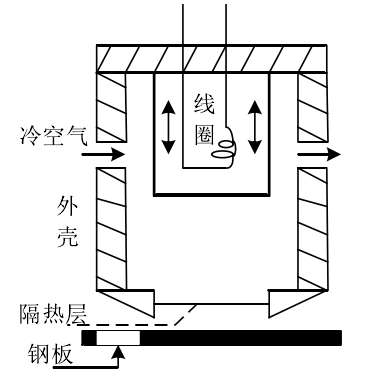
\includegraphics[width=6cm]{c2_eddy.png}
    \caption{电涡流检测原理}
    \label{fig:c2_eddy}
    \end{figure*}

    Helifa等\cite{Helifa2006Detection}设计了一种利用电涡流技术检测裂纹的方法,其方法的目标优化并选择在钢板上检测缺陷的最优电涡流线圈操作参数,首先是确定了使背景信号最小的操作参数来尽量降低背景信号对缺陷信号的干扰,之后通过在真实带缺陷钢板上的实验模拟出了缺陷区域的激励信号并建立了不同形状和大小的缺陷与阻抗平面上的信号的对应关系。其测试流程如图\ref{fig:c2_test_chian}所示:

    \begin{figure*}[!h]
    \centering
    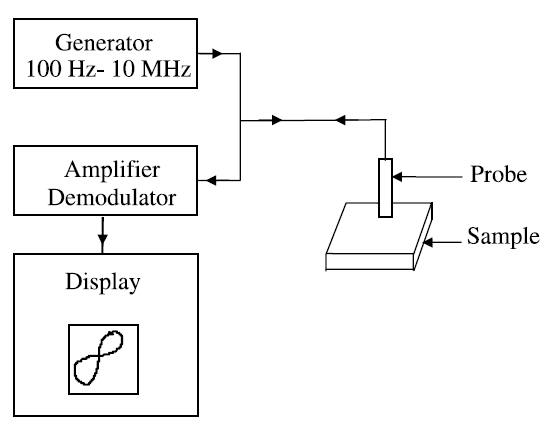
\includegraphics[width=6cm]{c2_test_chain.png}
    \caption{电涡流探伤检测流程}
    \label{fig:c2_test_chian}
    \end{figure*}

    宋凯等\cite{宋凯2015钢管磁特性对涡流检测影响的研究进展}整理并总结了目前使用电涡流技术在钢管无损缺陷检测的应用,阐述了钢管电涡流检测的机理和方法,分析并讨论了影响电涡流检测信号的缺陷漏磁场和缺陷区域畸变的磁导率等磁特性因素,最后总结了当前研究的发展趋势。

    电涡流检测法适用于检测中厚板材表皮与基层的阻流缺陷,该方法需要较大的电流激励才能达到预期的识别效果,因此能耗较大。另外,借助电涡流技术获得热图像必须具备待测板坯保持均匀温度场的前提,且有足够的时间让缺陷充分暴露,毫无疑问这对于高速度、快节奏、强水冷的热轧带钢生产线来讲是无法满足的。而且,使用电涡流检测技术容易受到电涡流探测器本身提离效应的约束,对激励信号的要求也比较高,因此目前国内外在高温连铸坯缺陷检测方面的电涡流检测方法尚未有突破进展。

    1990年,挪威的Elkem首次将红外检测技术用于连铸板坯表面缺陷检测。其系统的工作原理可参考图\ref{fig:c2_infrared},其主要思路是在连铸坯的生产线上装配高频的感应线圈,在满足高频感应的趋肤效应穿透深度小于1mm的情况下,当待检测连铸坯通过感应线圈时在其表面会感生出电流,遇到缺陷区域时,缺陷区域的凹陷或突出部分会产生感应电流,电流路径的延长使单位长度表面上的电能消耗增加,进而使得存在缺陷的连铸坯表面处的局部温度上升,这种局部的温度上升会被四周预装的红外扫描仪获得,从而达到识别钢坯表面缺陷的目的\cite{Vascotto1996High}。 在铸坯表面裂纹和细小孔洞的研究工作中,冈本芳三等\cite{Ooka1988Detection} 学者证明了红外方法的缺陷检测分辨力优于基于X射线检测和超声波探伤的方法。然而,由于缺陷的平均深度、线圈工作频率、感应线圈的宽度、特定的输入电能、钢坯的运动速度、被检钢坯的电性能和热性能以及环境干扰等诸多因素共同决定了缺陷和温升的对应关系,因此红外检测方法对条件依耐性强以及检测稳定性较差,只能局限于离线小范围的应用,难以在环境较为恶劣的热轧带钢生产线大范围推广。

    \begin{figure*}[!h]
    \centering
    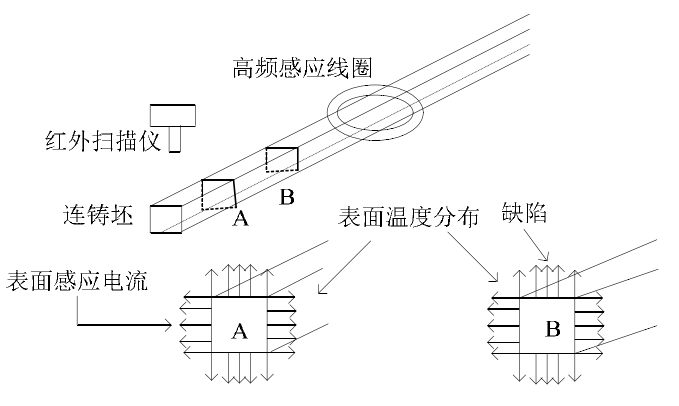
\includegraphics[width=12cm]{c2_infrared.png}
    \caption{红外检测原理}
    \label{fig:c2_infrared}
    \end{figure*}

    漏磁检测法的主要原理是漏磁通密度正比于缺陷体积,所以可以由漏磁通的密度来判断缺陷的大小和种类。在直流磁场中,钢坯被磁化且生成轴向饱和磁场。若钢坯有缺陷,磁通道的改变引起漏磁场的扩散,传感器能把泄露的磁力线检测出来,从而检测出钢坯缺陷的大小。漏磁检测方法的检测原理如图\ref{fig:c2_flux_leakage}。 漏磁检测法除了能检测钢坯表面的缺陷外,还可检测出钢坯内部微小的缺陷,其对于温度要求不高,检测精度高,廉价,但是其不适用于钢坯表面粗糙度的检测,也不能对大量的表面缺陷检测及分类。

    \begin{figure*}[!h]
    \centering
    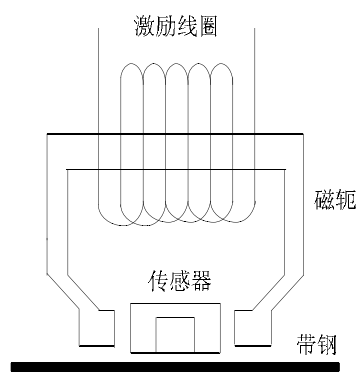
\includegraphics[width=6cm]{c2_flux_leakage.png}
    \caption{漏磁检测原理}
    \label{fig:c2_flux_leakage}
    \end{figure*}

    \section{基于RGB图像的方法}
    \esection{RGB Image based Method}
    相比较于传统无损检测方法,基于RGB图像的方法对钢板自身的物理特性如温度、密度、表面粗糙度等没有要求,并且在检测速度上也有较大优势,这类方法采用CCD摄像机采集钢板表面图像,然后通过图像处理和分析提取出图像特征进行缺陷的提取和分类。

    重庆大学的欧阳奇等\cite{欧阳奇2007高温连铸坯表面缺陷的机器视觉无损检测}针对高温连铸坯表面缺陷无法在线检测的问题,构建了一个连铸坯表面缺陷检测系统,该系统对采集的钢板表面图像进行灰度分析来检测是否存在缺陷,其首先对图像进行平滑滤波以消除噪声,然后对图像进行边缘检测来提取图像边缘,最后对边缘图像进行轮廓搜索将图像上所有的缺陷区域进行标记。

    北京交通大学的王建等\cite{王健2016基于图像分割的钢板表面缺陷识别}采用基于图像分割的方法来检测钢板表面的缺陷,该方法首先对图像进行预处理去除噪声,然后基于图像灰度统计信息的不同,采用了两种图像分割模型,当图像的灰度信息分布均匀时,采用C-V模型对图像进行分割,当图像的灰度信息分布不均匀时,则采用H-T-B模型对图像进行分割,通过这两种模型的组合应用可以对钢板的各类表面缺陷进行检测,获取缺陷区域。其检测的流程图如图\ref{fig:c2_segment_flow_chart} 所示:

    \begin{figure*}[!h]
    \centering
    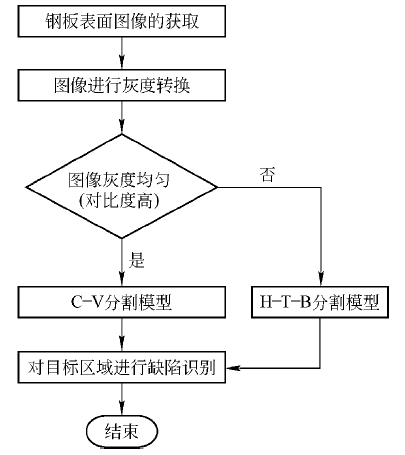
\includegraphics[width=6cm]{c2_segment_flow_chart.png}
    \caption{基于图像分割的缺陷检测流程图}
    \label{fig:c2_segment_flow_chart}
    \end{figure*}

    华中科技大学的刘思等\cite{刘思2011复杂背景下钢板表面缺陷检测的图像增强方法}采用了一种图像增强的办法来提升算法的缺陷检出性能,相较于传统的图像增强算法,该算法能够有效地显示出图像底层的结构特征。该方法首先计算像素的灰度平均值,然后采用均值量化方法将各个像素的灰度值量化为0或者1,接着将量化值输出分解到2个节点中。相比较于直方图均衡化还有分段拉伸,该算法显示出更优的图像增强性能。

    基于RGB图像的方法大部分是在空间域进行操作,主要是提取集合特征、纹理特征、灰度特征还有形状特征等进行缺陷的识别。另外,也有一些学者采用频域变换的方法将图像变换到时域以提取特征,常用的时域变换有Fourier变换、wavelet变换和Gabor变换等。

    中国地质大学的周新星等\cite{周新星2012基于独立成分分析的表面缺陷特征提取与识别方法}采用了一种基于时域变换的方法对钢板表面缺陷进行特征提取和识别,作者首先使用独立成分分析(ICA)和拓扑独立成分分析(TICA)从缺陷集中自适应地估计出基函数和滤波器,这些基函数适应于缺陷图像的特点,然后用于基函数对应的滤波器对钢板图像进行滤波操作,提取滤波响应作为特征向量,最后使用支持向量机对样本进行分类识别。该方法使用的基函数如图\ref{fig:c2_base_function}所示,从左至右依次为ICA 基函数和TICA基函数。该方法建立在对缺陷集无监督学习的基础上,能够自适应地提取缺陷图像的显著特征,且计算简单,可并行处理。该方法所使用的ICA 算法从盲源分离问题发展而来的基于信号高阶统计特性的分析方法,而TICA 则是ICA 的扩展方法。它们用于图像数据时,通过建立观测图像的统计生成模型对图像进行无监督学习,自适应地估计基函数和滤波器,从而用模型中的元素给出图像的表示。

    \begin{figure*}[!h]
    \centering
    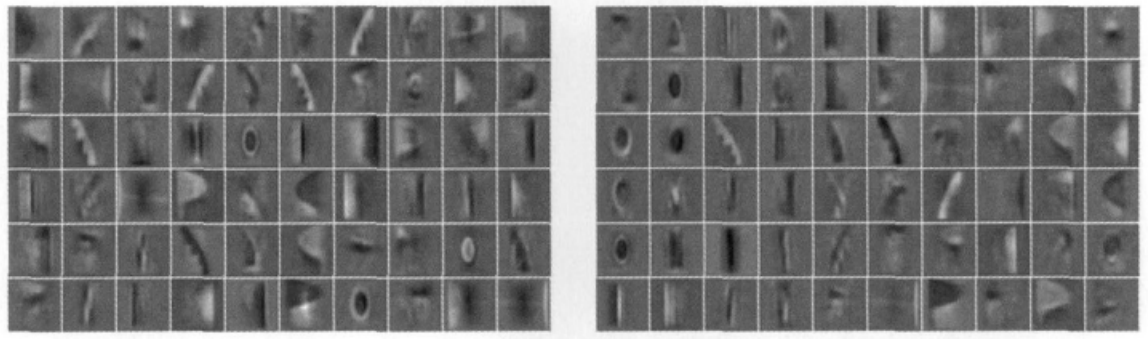
\includegraphics[width=12cm]{c2_base_function.png}
    \caption{缺陷基函数示意图}
    \label{fig:c2_base_function}
    \end{figure*}

    浦项科技大学的Jeon等\cite{Jeon2014Defect}提出了一种基于小波重建的钢板表面缺陷检测算法,该算法首先对钢板图像进行多次独立小波分解,然后对每一层小波分解出的不同分量的信号使用不同的权重加权,然后再将加权后的分量重建成一张新的钢板图像。带权重的二维小波重建的过程如图\ref{fig:c2_wavelet}所示。相比较于原图像,由于在重建的过程中对不同的分量使用了不同的权重,所以重建后的图像更多地保留了原图像的高频信息。接着,该方法对重建后的图像进行双阈值分割,双阈值分割的高低阈值都是根据图像的灰度均值以及标准差来确定的,双阈值分割使用高低阈值分别对图像进行二值化,然后对于每个低阈值分割出的连通区域,若其包含了任一高阈值分割出的连通区域,将其保留,否则抛弃。双阈值分割比一般的阈值分割相比有更高的查全率,并且缺陷轮廓更为完整。分割出缺陷区域后,该方法提取出缺陷的颜色和形态学特征使用支持向量机对缺陷进行分类。

    \begin{figure*}[!h]
    \centering
    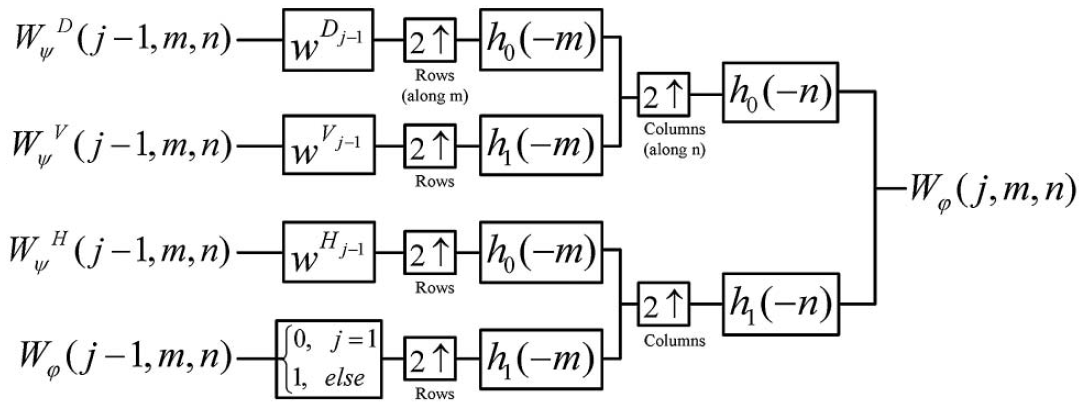
\includegraphics[width=12cm]{c2_wavelet.png}
    \caption{二维加权小波重建示意图}
    \label{fig:c2_wavelet}
    \end{figure*}

    \section{基于深度图像的方法}
    \esection{Depth Image based Method}
    目前深度图像被大量应用于行人检测、步态识别、三维目标识别等领域,但是利用深度图像进行缺陷检测的方法还较少,还没有形成一种典型的流程。相比较于RGB图像,深度图像有先天的优势,首先深度图像不存在RGB图像中反光、模糊、背景复杂等问题,并且由于钢板表面存在氧化铁皮、水膜、黑斑等伪缺陷,使用基于RGB图像的检测方法很难将其检测出来,因为这些伪缺陷在形态和颜色上都与缺陷较为相似,然而这些伪缺陷往往并不具有深度信息,所以在深度图像上往往不会表现出来。

    重庆大学的赵立明等\cite{赵立明2010连铸热坯表面缺陷激光扫描成像三维量化检测方法}设计了一种连铸坯表面缺陷三维量化系统,通过激光扫描成像获取连铸坯表面的深度图像并使用了一些图像处理的技术从深度图像中检测出缺陷。然而作者将深度图像进行灰度化处理,将深度图像当做灰度图像来使用,其检测方法本质上与基于RGB图像的方法类似,并没有真正利用到深度图像的三维特性,与基于RGB图像的方法相比,作者的方法主要还是成像方式不同。

    Zhang等\cite{Zhang2014Continuous}设计了一种钢板表面深度检测系统,作者将光栅投影方法、相位控制方法和时间相位展开方法结合起来检测连铸坯表面的深度信息。文章中显示用该方法检测出的深度图像较为平滑并且对各种缺陷的深度检测适应性较好,该系统的设计如图\ref{fig:c2_zhang}所示,该系统主要包括一台工作站、一个CCD面阵相机和一个数字控制液晶显示投影仪,投影仪能够计算受控结构光,然后通过光学透镜单元将它们投影到目标表面上。该系统主要目标是尽可能准确地测量钢板表面的深度信息,对于提取到深度信息之后,如何利用深度图像提取缺陷,文章中并没有讨论。

    \begin{figure*}[!h]
    \centering
    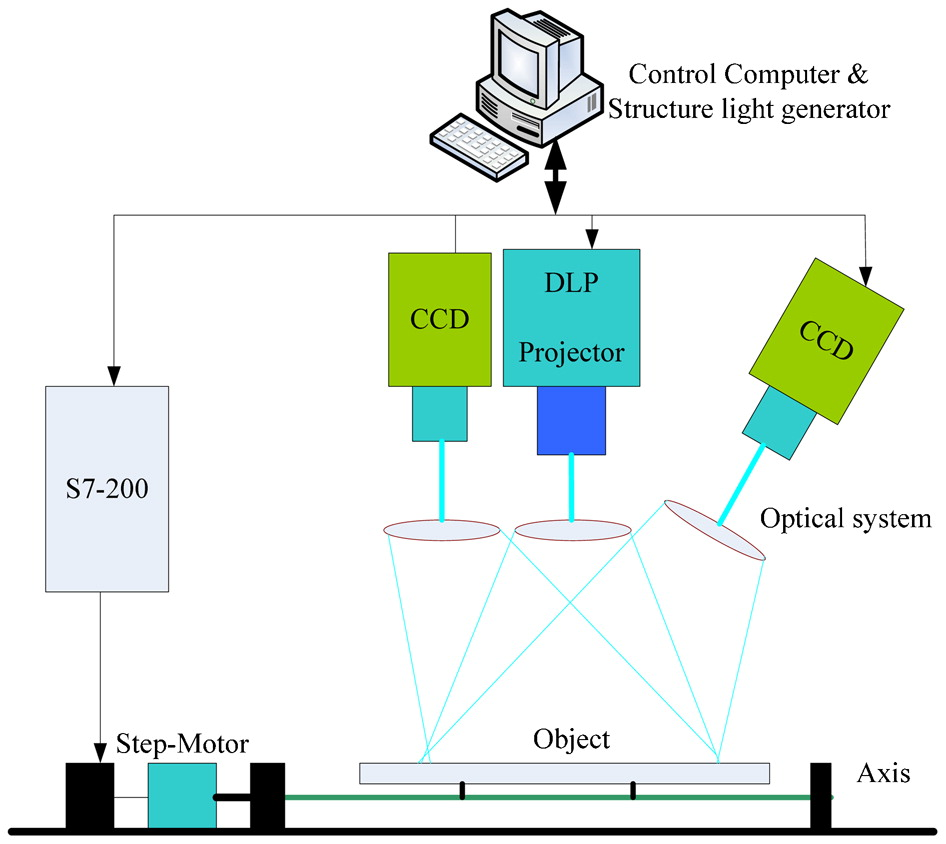
\includegraphics[width=12cm]{c2_zhang.png}
    \caption{系统设计图}
    \label{fig:c2_zhang}
    \end{figure*}

    Landstrom等\cite{Landstrom2012Morphology}提出了一种基于形态学操作的钢板表面裂纹提取算法,作者使用激光三角测量的方法获取了钢板表面深度图像。该方法对三维数据进行了一系列预处理,首先需要确定钢板区域,然后对三维数据进行斜率补偿,接着补齐三维数据中的缺省值,最后使用中值滤波去除噪声,由于一般的三维成像获得的三维数据质量并不高,所以进行这些预处理十分有必要。预处理结束后采用了多种形态学算子来对图像进行形态学操作,接着结合多种形态学操作的计算结果并使用阈值分割的策略获得最终缺陷连通区域,该方法对于裂纹的检测和分类准确率较高,其预处理阶段使用的斜率补偿等方法利用到了深度图像的特点,但是该方法所使用的形态学操作过程主要是针对裂纹这一种缺陷来设计的,对于其他类型的缺陷检出情况如何,作者并没有给出实验结果。

    zhao等\cite{Zhao2014Defect}设计了一个使用成对CCD传感器的连铸坯表面缺陷检测系统,简称DSI,作者使用激光扫描仪和CCD面阵相机同时获取钢板表面的深度图像和灰度图像,其设计的系统如图\ref{fig:c2_DSI_system}所示,该系统使用一个线阵CCD 相机和线阵激光发射器来获取钢板深度数据,另外使用一个面阵CCD相机来获取钢板的灰度图像。作者构建了一个算法将深度图像和灰度图像结合起来检测钢板表面缺陷。为了便于计算,作者首先使用基于互信息的方法将灰度图像和深度图像进行了配准,保证两个图像的像平面是完全对齐的,接着作者根据深度图像中的深度信息定位了一些缺陷种子点,然后根据这些种子点检测除了一些候选的感兴趣区域,接着使用iterative relative fuzzy connectedness 图像分割方法\cite{Udupa2014Body, Udupa1996Disclaimer} 将缺陷区域分割出来。该方法的一大特点就是将深度图像和灰度图像结合起来检测缺陷,由于使用了深度图像,该方法能够有效地抑制伪缺陷例如:氧化铁皮、水膜和黑斑等等,这些伪缺陷对于基于RGB 图像的方法来说往往是一个较大的挑战。另外,该方法不仅能够将缺陷检测出来,还能够准确地提取缺陷部分的轮廓。

    \begin{figure*}[!h]
    \centering
    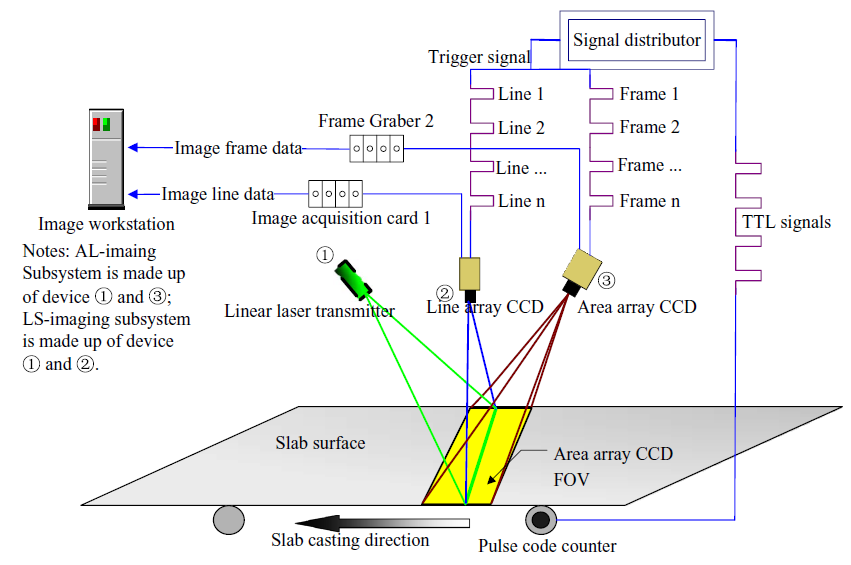
\includegraphics[width=12cm]{c2_DSI_system.png}
    \caption{DSI系统设计图}
    \label{fig:c2_DSI_system}
    \end{figure*}


    \section{本章小结}
    \esection{Brief Summary}
    本章中,主要对现有的连铸坯表面缺陷检测方法进行了整理和总结,现有的连铸坯表面缺陷检测方法主要分为传统无损方法、基于RGB图像的方法和基于深度图像的方法。传统无损方法其主要使用一些钢板的物理特性,通过钢板对电、热、磁等反应的变化来探测缺陷,这些方法往往存在一些局限性,并且方法的实时性不高。基于RGB图像的方法是目前连铸坯表面缺陷检测的研究热点,这些方法主要是使用CCD相机采集钢板灰度图像,然后使用一些图像处理的手段来检测缺陷位置,然而这些算法对于伪缺陷的误检率较高。基于深度图像的方法主要是使用钢板的深度图像来检测缺陷,利用深度信息能够有效地检测出缺陷并排除伪缺陷。


        % multiple1902 <multiple1902@gmail.com>
% intro.tex
% Copyright 2011~2012, multiple1902 (Weisi Dai)
% https://code.google.com/p/xjtuthesis/
%
% It is strongly recommended that you read documentations located at
%   http://code.google.com/p/xjtuthesis/wiki/Landing?tm=6
% in advance of your compilation if you have not read them before.
%
% This work may be distributed and/or modified under the
% conditions of the LaTeX Project Public License, either version 1.3
% of this license or (at your option) any later version.
% The latest version of this license is in
%   http://www.latex-project.org/lppl.txt
% and version 1.3 or later is part of all distributions of LaTeX
% version 2005/12/01 or later.
%
% This work has the LPPL maintenance status `maintained'。
%
% The Current Maintainer of this work is Weisi Dai。
%

\chapter{基于显著性图的缺陷检测算法}
\echapter{Saliency based Defect Detection Method}
图像显著性提取即将图像中视觉最突出的部分与其他区域划分开来,自从1998年Itti \cite{Itti1998A} 的工作以来,产生了大量的显著性映射方法\cite{Zhai2006Visual, Cheng2011Global, Achanta2008Salient, Achanta2009Frequency},图像显著性也广泛应用于图像压缩、编码、图像边缘和区域加强、显著性目标分割和提取等。使用显著性处理钢板表面的缺陷的基本原理是通过显著性方法对图像进行预处理,达到更好的突出缺陷区域的目的,并结合边缘检测等手段,最终将缺陷部分提取出来。
    \section{方法概述}
    \esection{Outline}
    由于生产条件和图像采集等诸多因素的影响,导致目前基于机器视觉的检测存在很多技术难点,如低对比度、图像质量过差、各类伪缺陷等。因此,本章提出了一种基于显著性的检测方法。

    基于显著性的缺陷检测方法先对输入的钢板图像进行显著性图的提取,通过这个步骤进行图像对比度的提升以及噪声的滤除,接着利用多个的显著性图所包含图像信息之间的差异去除黑斑,在这个步骤里同时使用了canny边缘检测\cite{Canny1986A}手段提取出缺陷区域的具体位置,当得到去除黑斑的边缘结果之后通过形态学膨胀将相邻的缺陷区域进行融合,最后进行缺陷的标注工作,具体流程如图\ref{fig:c3_flow_chart} 所示。

    \begin{figure*}[!h]
    \centering
    
\includegraphics[width=16cm]{c3_flow_chart.png}
    \caption{基于显著性的缺陷检测算法流程图}
    \label{fig:c3_flow_chart}
    \end{figure*}

    \section{显著性检测}
    \esection{Saliency Map Detection}
        \subsection{基于显著性图的对比度提升}
        \esubsection{Saliency Map based Contrast Enhancement}
        首先使用FT显著性检测方法\cite{Achanta2009Frequency}来处理钢板缺陷,主要因为该方法简单快速,符合缺陷检测的实时性要求,并且该方法能够显著提高缺陷区域与背景区域的对比度,对缺陷识别有很好的效果。

        该方法主要原理是通过使用两个高斯滤波器完成对图像不同频段的滤波操作,在实现上通过求取图像均值以及高斯滤波图像的距离完成显著性图的生成。具体来说,对于一幅输入图像,分别进行$lab$ 空间的均值操作以及高斯滤波操作,再通过公式( \ref{equ:c3_salient} )求取两幅图像对应位置的欧式距离就可以得到最终的显著性图。公式中$I_\mu$ 表示图像均值, $I_{whc}\left( {x, y} \right)$ 表示在$\left( {x, y} \right)$坐标位置的高斯滤波后的像素值。
        \begin{eqnarray}
        S\left( {x,y} \right) = \left\| {I_\mu - I_{whc}\left( {x, y}\right)} \right\|
        \label{equ:c3_salient}
        \end{eqnarray}
        针对本文中所提到的低对比度缺陷,该方法有很好的对比度提升效果,如图\ref{fig:c3_salient}所示,其中从左至右分别为原图、原图的边缘检测结果、显著性图、对显著性图做边缘检测的结果。对比直接使用原图进行边缘检测的结果我们发现使用显著性处理之后的图像检测到的边缘更加完整,噪声更少,但是在这里有必要说明的一点是提取显著性图时并非直接使用公式,而是使用了改进的显著性检测,这部分内容将会在接下来的章节详细讲述。

        \begin{figure*}[!h]
        \centering
        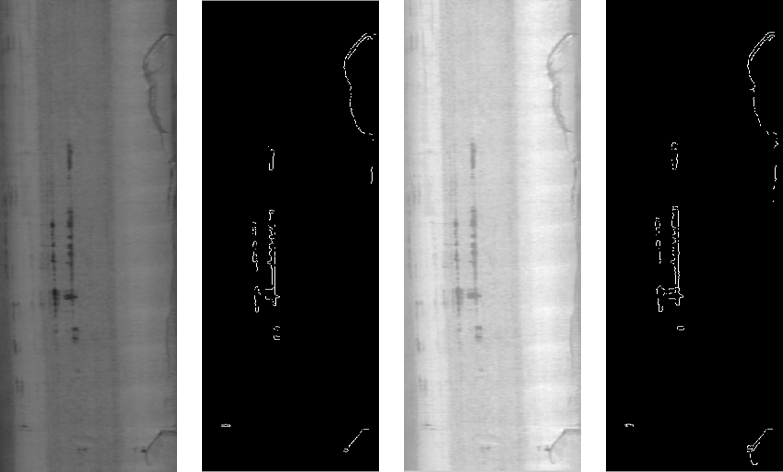
\includegraphics[width=16cm]{c3_salient.png}
        \caption{显著性检测对缺陷检测的提升效果}
        \label{fig:c3_salient}
        \end{figure*}

        \subsection{改进的显著性检测}
        \esubsection{Improved Saliency based Detection}
        上述提到的检测中,黑斑部分也作为一部分缺陷进行了检测,但是实际生产过程中,黑斑是作为一种伪缺陷并不需要进行检测,本节将使用一种改进的显著性检测方法去除这种伪缺陷对检测结果的干扰。

        公式中的$I_\mu$代表图像的均值,很显然在一副图像中大面积的背景区域对于图像的均值起着决定性的作用,这也是为什么直接使用公式对图像进行处理时如图\ref{fig:c3_multi_salient}中$\lambda = 1$的情况,背景区域将会变为全黑,基于此我们做一个变形:
        \begin{eqnarray}
        S\left( {x, y} \right) = \left| {\lambda * I_\mu - I_{whc}\left( {x, y}\right)} \right|, \lambda \in \left[ {0, 1} \right]
        \end{eqnarray}
        通过调整$\lambda$的取值,我们可以得到不同的显著性图,如图\ref{fig:c3_multi_salient}所示,当$\lambda$取值不同时,我们可以认为人为改变了图像的”背景“,相对应的”前景“区域也发生了变化,根据这种特点,我们可以容易得到图像中不同层次的内容,也就可以将黑斑的区域从图像中剔除出来。

        \begin{figure*}[!h]
        \centering
        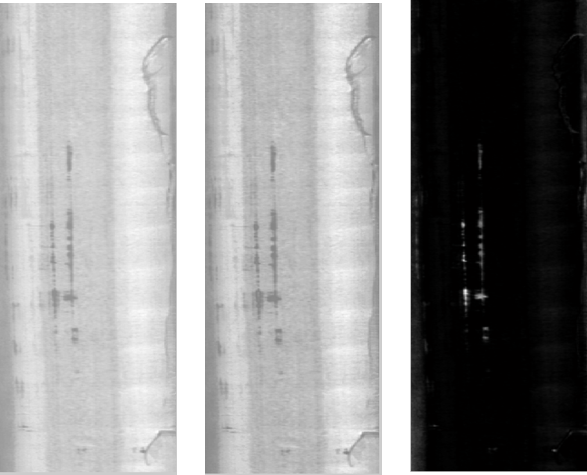
\includegraphics[width=16cm]{c3_multi_salient.png}
        \caption{使用不同$\lambda$的显著性检测效果,从左至右分别为$\lambda = 0.3$、$\lambda = 0.5$和$\lambda = 1$}
        \label{fig:c3_multi_salient}
        \end{figure*}

        对于一幅输入图像,分别对图像使用两个$\lambda$ 取值不同的显著性提取,一方面设$\lambda$为0.5得到同时包含缺陷和黑斑并且对比度进行加强的图像,接着对显著性图像进行canny边缘提取,得到备用的缺陷图像;另一方面使用$\lambda$ 为1进行显著性提取,使得图像只包含最显著的目标,即黑斑区域(实际上在一幅图像里,黑斑区域较其他区域具有明显的显著性目标特征),针对这幅图像,我们使用一个简单的二值化操作将黑斑的区域提取出来,由于可能检测到的黑斑区域并不十分完整,因此采取形态学膨胀的手段使得黑斑包围的面积更加完全,即使超出了原有黑斑的区域,在接下来的减除操作里,也可以避免这种误差造成的影响。在得到了上述两幅图像之后,进行作差工作,具体的原理如公式( \ref{equ:c3_black_spot_1} ) ( \ref{equ:c3_black_spot_2} ) 所示,$I_e$ 表示边缘检测的结果,$I_b$ 表示二值化和膨胀后的结果,作差后的结果$I_m$ 即为去黑斑后的中间结果图像。
        \begin{eqnarray}
        I_m = \Delta \left( {I_e - I_b} \right)
        \label{equ:c3_black_spot_1}
        \end{eqnarray}
        其中,函数$\Delta$为阶跃函数,其函数形式为:
        \begin{eqnarray}
        \Delta \left( x \right) = \left\{ \begin{matrix}
        0,&x<=0\\
        1,&x>0
        \end{matrix}\right.
        \label{equ:c3_black_spot_2}
        \end{eqnarray}
    \section{边缘提取}
    \esection{Edge Detection}
    在获得显著性图像之后,对图像进行边缘提取获得边缘图像。图像边缘是指邻域内像素的灰度值存在较大变化的像素点的集合,在频域上表示了图像的高频区域,在灰度图像上反映出了图像中灰度值的不连续性。图像的边缘检测\cite{Gonzalez2010Digital}能够大幅减少数据量,并且剔除不相关信息,保留图像中最重要的结构信息。边缘检测的实际目标是利用某种算法来提取图像中目标与背景之间的边缘线,通常可以由图像的一阶导数的最大值或者二阶导数的过零点检测得到图像边缘。常用的一阶导数有Roberts、Prewitt、Sobel 等\cite{Heath1998Comparison}梯度算子;基于二阶导数过零点检测的边缘检测算子中最典型的是由 Marr等提出的LoG算子\cite{Gonzalez2010Digital}。这些检测方法都是基于局部滑动窗的方法,其检测效果一般不理想,检测出的边缘并不完整存在断裂情况,并且往往会产生较多噪声。

    该方法使用Canny边缘检测算法\cite{Canny1986A}来提取边缘图像,相比较于其他的边缘检测算子,Canny算子具有较大的信噪比和较高的检测精度。Canny边缘检测算法的目标是找到一个最优的边缘检测算法,其认为最优边缘检测的目标是:

    1)最优的检测:即算法能够尽可能多的找出图像中的实际边缘;

    2)最优的定位:即算法标识出的边缘要尽可能与图像中的边缘位置一致;

    3)最小的响应:即图像中的边缘应最多被标识一次,并且尽可能减少噪声的误检情况:

    Canny边缘检测方法的一般步骤如下所示:

    1)计算图像与高斯平滑滤波器的卷积结果;

    2)使用一阶梯度算子计算图像的水平方向梯度图和垂直方向梯度图;

    3)根据水平方向梯度图和垂直方向梯度图计算梯度幅值和方向;

    4)使用非极大值抑制,细化梯度图像,只保留梯度幅值变化最大的那个点。

    使用Canny边缘检测方法在显著性图像上提取边缘来获取缺陷候选项,Canny边缘检测的效果如图所示,从左至右依次为原图、显著性图像、边缘图像。

    \begin{figure*}[!h]
    \centering
    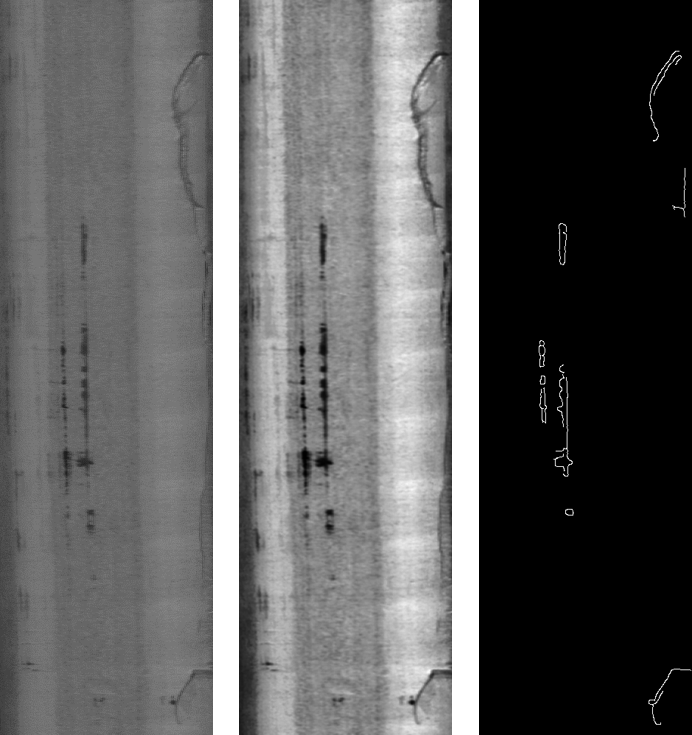
\includegraphics[width=16cm]{c3_edge_detect.png}
    \caption{Canny边缘检测效果图}
    \label{fig:c3_edge_detect}
    \end{figure*}


    \section{形态学操作}
    \esection{Morphology Operation}
    在获取边缘图像之后,需要使用形态学操作\cite{Gonzalez2010Digital,Wilkinson2009Mathematical}将断裂和或者比较接近的边缘连接起来,避免检测的缺陷结果过多。形态学操作是一门以集合论为基础的新兴研究方向,主要被用来分析和描述信号的几何形态。其基本思想是利用设计好的结构元素对信号进行各种形态学处理,能够删除掉不相关的信息,并保留信号的主要形状,作为探针的结构元素可以携带知识,如方向、大小、颜色等信息,不同的结构元素可以得到不同的结果。

    在算法中,主要使用了正方形5x5的形态学算子对边缘图像进行膨胀操作,膨胀会“粗化”二值图像中的物体,用来桥接裂缝。边缘检测出的边缘图像中连通区域较多,可能一个缺陷部分会断裂成多个连通区域,所以膨胀操作用来将这些断裂的情况重新连接起来,接着使用孔洞填充算法填补连通区域内部的孔洞,得到最终的检测结果。

    \section{实验结果}
    \esection{Experimental Results}
        \subsection{数据集与评价方法}
        \esubsection{Data-set and Evaluation Protocol}
        为了验证本方法的有效性,搜集整理了113张带黑斑低对比度缺陷的钢板图像制作了该类缺陷类型测试集,钢板图像的分辨率为289x998,同时为了验证本方法同样适用于其他类型缺陷的检测,搜集整理了125张结疤类型缺陷和100张压痕类型缺陷,并且对每一张缺陷图像都进行了缺陷区域的groundtruth标记,表是对测试集的数据内容总结,图\ref{fig:c3_defect_type} 展示了三种缺陷类型。

        \begin{figure*}[!h]
        \centering
        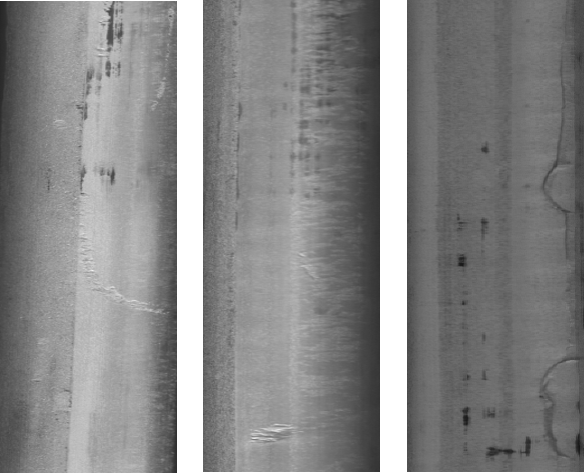
\includegraphics[width=16cm]{c3_defect_type.png}
        \caption{三种不同的缺陷类型,从左至右以及为结疤、压痕和带黑斑低对比度缺陷}
        \label{fig:c3_defect_type}
        \end{figure*}

        \subsection{实验结果与分析}
        \esubsection{Experimental Results and Analysis}
        实验环境为3.10GHZ Intel Core i5,4g内存,win7系统,使用MATLAB和c++代码进行实验。总的检测结果使用以下指标来衡量:查全率、查准率、和F值。

        基于显著性的方法首先对图像进行高斯滤波器进行滤波操作,然后将图像从RGB 空间转换到LAB空间,接着提取出图像的显著性图,然后对显著性图进行canny 边缘检测提取边缘图像,最后对边缘图像进行形态学操作。使用MATLAB 语言实现的部分代码如下:

        \lstinputlisting{code/xianzhuxing.m}

        为了说明本文提出的缺陷检测方法的有效性,使用本文的方法与自适应平滑滤波canny算子检测方法\cite{Canny1986A}以及基于kirsch边缘的缺陷检测方法\cite{李伟2016热态高速线材表面缺陷检测系统研究与实现} 做了对比试验,对于三种缺陷类型的实验结果分别如下表所示:

        \begin{table*}[!h]
        \centering
        \caption{结疤类型缺陷检测结果}
        \label{tbl:c3_salient_result_1}
        \begin{tabularx}{\columnwidth}{>{\centering\arraybackslash}X >{\centering\arraybackslash}X >{\centering\arraybackslash}X >{\centering\arraybackslash}X}
        \toprule
        方法 & 查全率 & 查准率 & F值 \\
        \midrule
        基于显著性图 & 0.9580 & 0.7446 & 0.8382 \\
        Canny边缘检测 & 0.8993 & 0.2487 & 0.3896 \\
        kirsch边缘检测 & 0.7625 & 0.6276 & 0.6885 \\
        \bottomrule
        \end{tabularx}
        \end{table*}

        \begin{table*}[!h]
        \centering
        \caption{压痕类型缺陷检测结果}
        \label{tbl:c3_salient_result_2}
        \begin{tabularx}{\columnwidth}{>{\centering\arraybackslash}X >{\centering\arraybackslash}X >{\centering\arraybackslash}X >{\centering\arraybackslash}X}
        \toprule
        方法 & 查全率 & 查准率 & F值 \\
        \midrule
        基于显著性图 & 0.8803 & 0.7923 & 0.8340 \\
        Canny边缘检测 & 0.8531 & 0.3927 & 0.5378 \\
        kirsch边缘检测 & 0.8536 & 0.6313 & 0.7261 \\
        \bottomrule
        \end{tabularx}
        \end{table*}

        \begin{table*}[!h]
        \centering
        \caption{带黑斑低对比度类型缺陷检测结果}
        \label{tbl:c3_salient_result_3}
        \begin{tabularx}{\columnwidth}{>{\centering\arraybackslash}X >{\centering\arraybackslash}X >{\centering\arraybackslash}X >{\centering\arraybackslash}X}
        \toprule
        方法 & 查全率 & 查准率 & F值 \\
        \midrule
        基于显著性图 & 0.8673 & 0.4959 & 0.6310 \\
        Canny边缘检测 & 0.5877 & 0.2084 & 0.3076 \\
        kirsch边缘检测 & 0.2113 & 0.3987 & 0.2762 \\
        \bottomrule
        \end{tabularx}
        \end{table*}

        实验结果表明在加入了显著性方法之后,对三类缺陷的检测结果均有提升,带黑斑低对比度类型缺陷尤其明显。虽然基于显著性的方法相对于canny算子检测方法对于结疤和压痕两类缺陷的查全率提升并不明显,但是在查准率方面提升很大,这说明在其他两类缺陷中使用原图进行canny边缘检测时,是通过较高的误检率来提高检测缺陷的数量,这在工业生产中仍然会造成相当多的问题,而显著性方法查全率和查准率都较高,整体的性能明显优于单纯使用边缘检测的方法。同时,需要说明的一点是由于带黑斑低对比度图像中存在的黑斑数量过多、灰度值分布范围较广、黑斑形状多变等因素导致黑斑伪缺陷很难被完全滤除,这也导致了实验结果的查全率不是特别高,但是黑斑误检为缺陷的情况已经大幅度降低,相对于其他两种方法的效果已经有了很大的提升。

        在时间方面,自适应平滑滤波canny算子检测方法平均耗时为25ms,基于kirsch 边缘缺陷检测方法平均耗时为18ms,基于显著性的缺陷检测方法平均耗时为40ms,虽然基于显著性的缺陷检测方法相对于其他两种方法的耗时要相对长一些,但是该算法的时间性能已经完全可以满足工业生产的要求了。

        图\ref{fig:c3_salient_result}展示了使用自适应平滑滤波canny算子缺陷检测与基于显著性方法的缺陷检测方法的部分实验结果效果对比,可以看出在使用了改进的显著性检测进行对比度增强和去黑斑之后,检测的缺陷区域更加完整,黑斑伪缺陷的误检大大降低,第二行检测的黑斑区域在第一行中对应的图像中几乎没有检测出来。

        \begin{figure*}[!h]
        \centering
        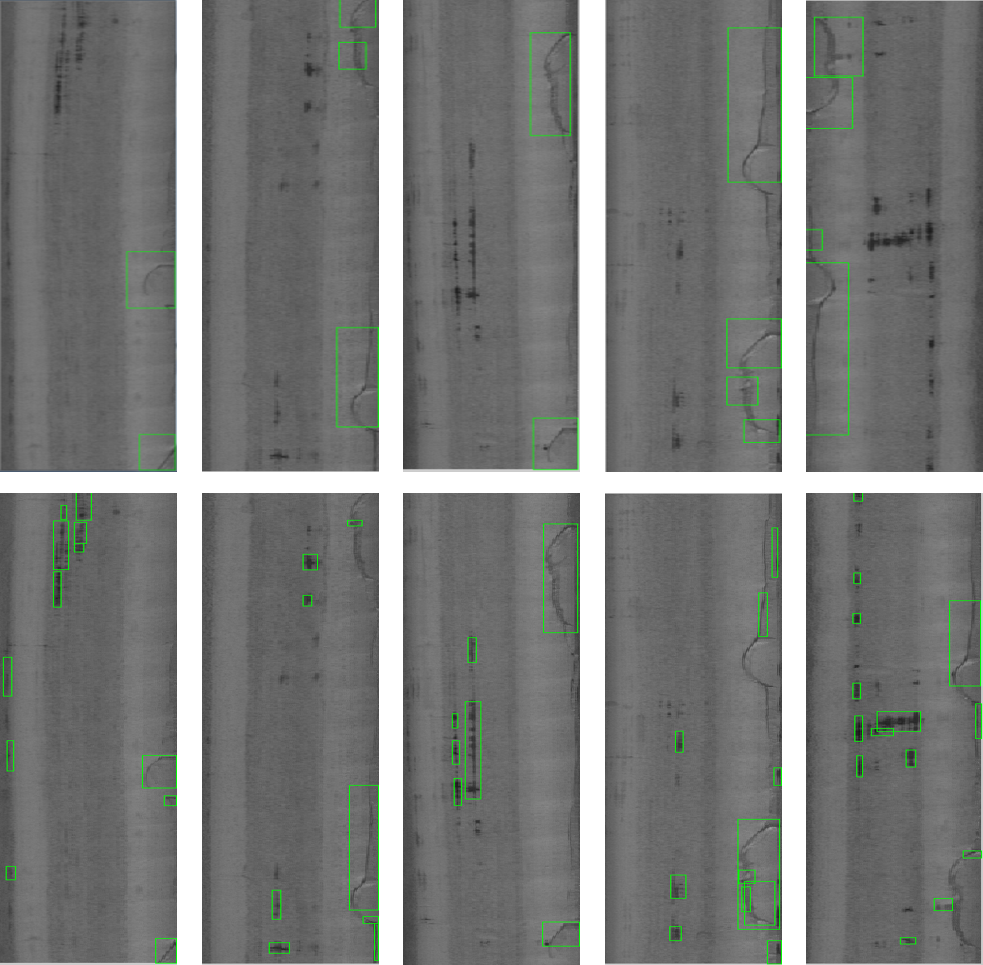
\includegraphics[width=16cm]{c3_salient_result.png}
        \caption{部分检测结果,从上之下依次为基于显著性图的方法和canny算子检测的实验结果}
        \label{fig:c3_salient_result}
        \end{figure*}

        综上实验结果,可以充分说明基于显著性的缺陷检测方法不仅对于低对比度带黑斑缺陷有很好的检测效果,对于其他类型缺陷同样具有良好的检测效果。
    \section{本章小结}
    \esection{Brief Summary}
    本章所提出的基于显著性的缺陷检测方法,很好的解决了目前基于机器视觉的低对比度带黑斑缺陷检测难点,通过该方法,检测出的缺陷更加完整,误检数量明显减少,由于结合了改进的显著性检测方法,去除了图像中黑斑伪缺陷对检测结果的干扰,同时,该方法检测速度快,完全符合缺陷检测中对时间性能的要求。当然,该方法仍有继续研究和改进的空间,如何更加完整的提取到缺陷区域、更加完全的去除黑斑,以及时间性能的进一步提高都将成为接下来的工作重点。


        % multiple1902 <multiple1902@gmail.com>
% intro.tex
% Copyright 2011~2012, multiple1902 (Weisi Dai)
% https://code.google.com/p/xjtuthesis/
%
% It is strongly recommended that you read documentations located at
%   http://code.google.com/p/xjtuthesis/wiki/Landing?tm=6
% in advance of your compilation if you have not read them before.
%
% This work may be distributed and/or modified under the
% conditions of the LaTeX Project Public License, either version 1.3
% of this license or (at your option) any later version.
% The latest version of this license is in
%   http://www.latex-project.org/lppl.txt
% and version 1.3 or later is part of all distributions of LaTeX
% version 2005/12/01 or later.
%
% This work has the LPPL maintenance status `maintained'.
%
% The Current Maintainer of this work is Weisi Dai.
%

\chapter{基于基准面拟合的缺陷检测算法}
\echapter{Datum Plane based Defect Detection Method}
由于伪缺陷的干扰以及RGB图像本身存在的低对比度和光照等问题,使用RGB图像较难从图像中准确地提取缺陷区域,目前钢板表面的缺陷大部分都具有深度信息,所以使用深度信息来检测缺陷是发现热态钢板表面缺陷的有效手段。本章方法利用深度图像拟合出钢板基准面,然后根据基准面以及原始深度图像获得缺陷种子点,最终在深度图像上使用基于种子点的图像分割算法分割出缺陷区域。
    \section{方法概述}
    \esection{Outline}
    该方法应用于钢板表面缺陷检测系统中,输入是3D相机采集到的深度图像,输出为缺陷的位置。钢板表面情况较为复杂,钢板表面本身一般并不平整,并且在钢板传输过程中可能存在抖动,另外在利用摄像头采集图像时,由于钢板表面的温度较高,钢板表面可能存在雾化效果。这些干扰因素都会影响采集到的深度图像,并最终使得基于深度图像的缺陷检测算法更加困难,本算法旨在保证系统稳定运行的前提下,尽可能提高缺陷的检出率,降低误检率。

    该方法是基于滑动窗的方法,首先对深度图像进行平滑处理,平滑处理的流程是:如果当前像素点的深度值大于邻域窗口内平均值与标准差之和,或者小于平均值与标准差之差则将该像素点的深度值修正为窗口内的平均值,否则,该像素点的深度值不变。

    接着对深度图像进行局部基准面拟合,拟合的方法类似于移动曲面拟合法,移动曲面拟合法是一种以待定点为中心的局部拟合方法,以每个待定点为中心,其定义一个局部函数去拟合周围的数据点。采用此方法拟合,在每个待定点的邻域上都可以单独求出一个拟合函数,通过拟合函数可以直接计算出待定点上的拟合值,这种计算方式比较灵活,并且拟合区域相对较小,可使周围数据点更好地发挥其控制作用。对于以待定点为中心的所有邻近点,选择一种曲面函数为拟合面,曲面函数可以采用一次函数、二次函数或者三次函数,选择不同的拟合函数对应不同的拟合精度。

    最后根据最小二乘法原理解出去曲面函数的系数得到拟合的基准面。基准面拟合结束后,对于图像中的每一个像素点都能够获得一个基准面深度值,然后我们利用基准面来生成种子点。若对于某个像素点,其基准面的深度值与原始深度值的差大于一个阈值,则被认为是一个种子点。获得种子点之后,最后就是在深度图像上使用SFM水平集的方法进行图像分割来提取最终的缺陷轮廓。

    基于基准面的缺陷检测算法一般流程如图\ref{fig:c4_flow_chart}所示,包括了基准面拟合,种子点提取,和基于种子点的图像分割。

    \begin{figure*}[!h]
    \centering
    
\includegraphics[width=16cm]{c4_flow_chart.png}
    \caption{基于基准面的拟合的缺陷检测流程图}
    \label{fig:c4_flow_chart}
    \end{figure*}

    \section{基准面拟合}
    \esection{Datum Plane Fitting}
    基准面拟合的思路主要受启发与海洋测绘领域对海平面的基准面测量\cite{孙学华2011海域无缝深度基准面的建立}。给定一副输入的深度图像,首先对其进行基准面拟合,拟合的目的就是找到钢板的基准面。这里采用的基准面拟合算法是使用滑动窗的局部基准面拟合算法。

    典型的曲面拟合方法主要有Shepard拟合法还有移动曲面拟合法,其中Shepard拟合法首先由气象学及地质学工作者提出,后来由Shepard的工作被称为Shepard方法,该方法在使用时无需解线性方程组,是大规模数据拟合方法中最简单、最典型的一种方法。其基本思想是将待定点的函数值定义为拟合半径范围内各数据点函数值的加权平均,各数据点的权重按其距待定点的距离计算,该方法主要存在的问题是:(1)如果很拟合半径较大,计算一个点,需要耗费很大的工作量;(2)权重函数仅由点的距离确定,没有考虑其他因素,如方向等;(3)在待定点附近的平坦点会出现微小扰动。之后Shepard对该方法的加权函数进行了改进,提出了一种局部逼近模型,该模型是一个分段函数,将拟合半径内的拟合区域分为两个环带,已知点的权按其距待定点的不同范围采用不同的权函数,保证越靠近待定点的已知点的权重越大,远离待定点的已知点的权迅速减小。该模型将拟合区域分区加权,把拟合精度与距离联系起来建立函数模型,一般适用于大面积、点位分布均匀的区域,能有效地对理论深度基准面变化复杂的区域进行拟合。在实际应用中要根据点位分布密度和面积选取合适的拟合半径。

    移动曲面拟合法是一种以待定点为中心的逐点内插法,它以每个待定点为中心,定义一个局部函数去拟合周围的数据点。采用此方法拟合,在每个待定点上都可单独求定一个拟合函数,直接得到待定点上的拟合值,计算比较灵活,并且拟合区域相对较小,可使周围数据点更好地发挥其控制作用。对于以待定点为中心的所有邻近点,选择一种曲面函数为拟合面,曲面函数可以采用一次函数、二次函数或者三次函数,选择不同的拟合函数对应不同的拟合精度。最后根据最小二乘法原理解出去曲面函数的系数得到拟合的基准面。

    我们的方法的类似于移动曲面拟合方法,假定滑动窗的窗口大小为$W_s$,首先对图像进行平滑处理,平滑处理的流程是:如果当前像素点的深度值大于邻域窗口内平均值与标准差之和,或者小于平均值与标准差之差则将该像素点的深度值修正为窗口内的平均值,否则,该像素点的深度值不变。邻域窗口的半径$W_n=\sqrt{W_s}$, 该流程的公式表达为:
    \begin{eqnarray}
    \left\{ \begin{array}{l}
    S\left( i \right) = {\mu _i},abs\left( {f\left( i \right) - {\mu _i}} \right) > {\sigma _i}\\
    S\left( i \right) = f\left( i \right),otherwise
    \end{array} \right.
    \end{eqnarray}
    其中$i$代表一个像素点,$S\left(i\right)$和$f\left(i\right)$分别代表该像素点的平滑后深度值和深度图像的深度值。$\mu_i$和$\sigma_i$分别代表该像素点邻域窗口内的深度平均值和标准差。

    平滑处理结束后,再将平滑后的深度数据使用最小二乘法进行三次多项式拟合,拟合后的三次函数即表示深度图像的基准面。

    基准面拟合的结果如图\ref{fig:c4_plane_fit}所示,从左至右依次为深度数据三维伪彩图、平滑后深度数据三维伪彩图、最终拟合出的基准面。

    \begin{figure*}[!h]
    \centering
    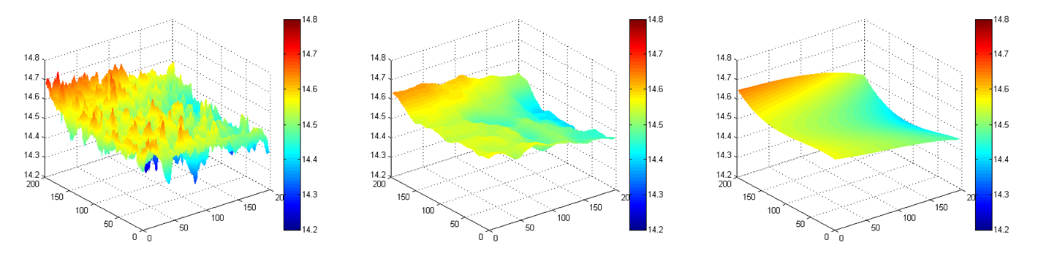
\includegraphics[width=16cm]{c4_plane_fit.png}
    \caption{基准面拟合效果图}
    \label{fig:c4_plane_fit}
    \end{figure*}

    \section{种子点提取}
    \esection{Seed Specification}
    基准面拟合结束后,对于图像中的每一个像素点都能够获得一个基准面深度值,然后我们利用基准面来生成种子点。若对于某个像素点,其基准面的深度值与原始深度值的差大于一个阈值,则被认为是一个种子点。种子点生成策略如下公式所示:
    \begin{eqnarray}
    S_d=\left\{i:d_{norm}\left(i\right)>f\left(i\right)+T_{depth}\right\}
    \end{eqnarray}
    其中$S_d$表示缺陷种子点集合,$i$表示一个像素点,$d_{norm}\left(i\right)$ 和$f\left(i\right)$分别表示该像素点的基准面的深度值和深度图像的深度值, $T_{depth}$ 是一个阈值,该阈值需要根据缺陷的深度定义来确定。
    \section{基于种子点的图像分割}
    \esection{Seed based Image Segmentation}
    获得种子点之后,下一步就是在深度图像上使用基于种子点的图像分割算法,可以采用的方法有很多,例如:Graph cut\cite{Boykov2001Interactive, Boykov2001Fast}、random walker\cite{Grady2006Random}、SFM 水平集\cite{Lankton2009Sparse}和Fuzzy connectedness\cite{Udupa2014Body, Udupa1996Disclaimer}等等。经过实验,我们选择SFM 水平集方法作为最后的分割算法,因为该方法的效果最好,能够有效的应对噪声。

    SFM水平集属于主动轮廓方法,主动轮廓图像分割方法能够迭代地演化一个轮廓从而尽可能一张图像分割成多个连通区域,达到图像分割的效果。SFM水平集的方法非常流行,主要是因为该类方法实现比较简单,并且能够拟合出足够复杂的模型。在SFM 水平集理论框架中,水平集轮廓可以理解为被包含在更高维度的函数中,比如一个二维平面中的轮廓$C$可以表示为三维空间中的函数$\phi$,按照惯例轮廓$C$可以表示成三维空间中函数$\phi$的零水平集,当$\phi<0$时,表示轮廓$C$的内部,当$\phi>0$时,代表轮廓$C$的外部区域。如图\ref{fig:c4_level_set}所示,这里给出一个例子,假设轮廓$C$ 是一个圆圈,那么对应的函数$\phi$的零水平集正好与轮廓$C$相匹配。

    \begin{figure*}[!h]
    \centering
    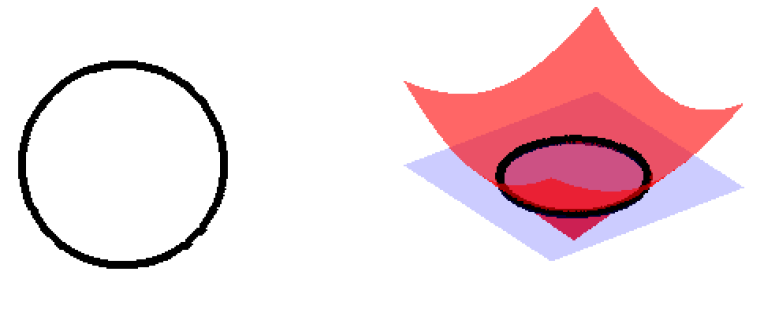
\includegraphics[width=16cm]{c4_level_set.png}
    \caption{SFM水平集理论示意图}
    \label{fig:c4_level_set}
    \end{figure*}

    SFM 水平集采用的是迭代的思路,基于局部信息不断扩大或者缩小水平集,相比较其他分割算法而言更为关注局部信息。SFM水平集算法通过不停的迭代修改0水平集的轮廓来最小化Chan-Vese能量函数\cite{Chan2001Active},Chan-Vese能量函数主要被用于主动轮廓模型领域,其函数形式如下:
    \begin{eqnarray}
    E=\int_{interior}\left({I-\mu_1}\right)^{2}+\int_{exterior}\left({I-\mu_2}\right)^{2}
    \end{eqnarray}
    SFM水平集分割算法结果如图\ref{fig:c4_SFM}所示,从左至右依次为深度图像三维伪彩图、提取的种子点图像、分割后的二值图像。

    \begin{figure*}[!h]
    \centering
    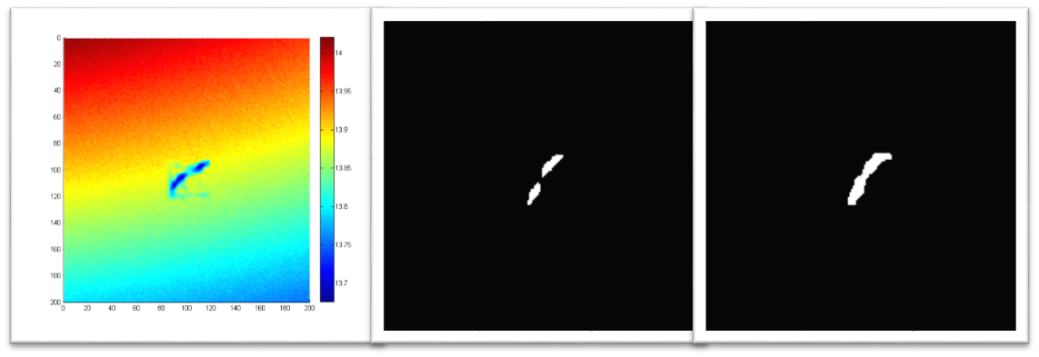
\includegraphics[width=12cm]{c4_SFM.png}
    \caption{SFM水平集分割算法效果图}
    \label{fig:c4_SFM}
    \end{figure*}

    \section{实验结果}
    \esection{Experimental Results}
        \subsection{数据集与评价方法}
        \esubsection{Data-set and Evaluation Protocol}
        目前采集到的钢板深度图像数据有限,为了能够对本文中提出的两种深度图像缺陷检测算法进行评价,利用真实的钢板深度图像我们采用人工合成的手段构建了一个钢板深度图像数据集。我们首先使用结构光3D扫描技术采集到一些带缺陷的钢板点云数据,然后将这些点云数据进行插值和裁剪处理转化为了深度图像。

        利用这些真实的带缺陷的钢板深度数据我们使用人工合成手段创建了一个深度图像数据集,该数据集一共有500张深度图像,图像的分辨率为1000x1000,缺陷数量总共有1489个。创建的流程主要为:

        1)根据真实钢板深度图像生成钢板模型;

        2)根据真实深度图像上的缺陷区域生成缺陷模型,另外也采用高斯函数生成了部分缺陷模型;

        3)随机选择钢板模型和缺陷模型,将钢板模型和缺陷模型组合起来生成合成深度图像。

        根据真实的钢板深度图像,首先随机提取100张1000x1000的子图,然后使用章节4.2中的基准面拟合方法拟合出这些子图的基准面,接着将这些基准面保存下来作为钢板模型。部分钢板模型的三维伪彩图如图\ref{fig:c4_steel_model}所示。

        \begin{figure*}[!h]
        \centering
        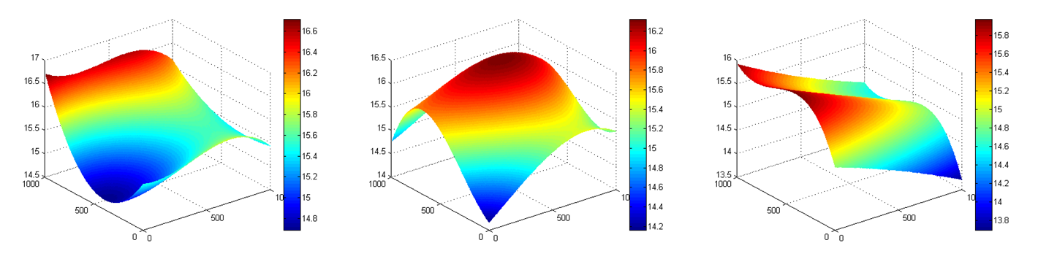
\includegraphics[width=16cm]{c4_steel_model.png}
        \caption{部分钢板模型三维伪彩图}
        \label{fig:c4_steel_model}
        \end{figure*}

        在真实的钢板深度图像上,我们使用人工标记的方法标记了缺陷区域,然后计算出这些缺陷区域与基准面的深度偏差,接着对深度偏差进行归一化,使得最大深度偏差等于缺陷的深度定义$D_{depth}$,然后归一化的深度偏差被保存作为缺陷模型。另外,我们也使用二维高斯函数生成了一些缺陷模型,最终一共生成了12 种缺陷模型。部分缺陷模型的三维伪彩图如图\ref{fig:c4_defect_model}所示:

        \begin{figure*}[!h]
        \centering
        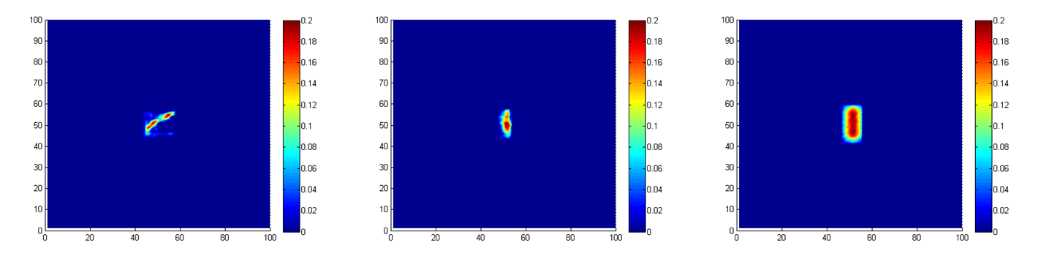
\includegraphics[width=16cm]{c4_defect_model.png}
        \caption{部分缺陷模型三维伪彩图}
        \label{fig:c4_defect_model}
        \end{figure*}

        最后,随机选择一个钢板模型和若干缺陷模型,对于每个缺陷模型,都采用参数随机的尺度变换和旋转变换来生成一个新的缺陷模型,尺度变换的尺度参数从0.5到2,步长为0.5,旋转变换的角度参数从0到360,步长为30。然后随机选择缺陷位置,将钢板模型减去缺陷模型获得带缺陷的钢板深度图像。

        对于检测算法检出的一个缺陷连通区域,我们使用连通区域包围盒的重叠率来判断检测是否成功,假定$R_p$为检测算法检测出的缺陷连通区域包围盒,$R_t$ 是已标记的缺陷连通区域包围盒,若$\frac{{R_p}\bigcap{R_t}}{{R_p}\bigcup{R_t}}>T_{overlap}$,即包围盒重叠率大于某个阈值则认为检测算法检出的该连通区域是一个缺陷。我们使用查全率、查准率和F 值来评价算法的最终检测效果。
        \subsection{实验结果与分析}
        \esubsection{Experimental Results and Analysis}
        我们使用Matlab语言实现了本文提出的两个深度图像缺陷检测算法,实验用的计算机配置为:Intel Xeon E3-1241 3.50GHz CPU、32GB内存、Windows 7操作系统。处理一张1000x1000的深度图像,基于基准面的方法平均处理时间为38s,使用了C++代码实现并增加多线程策略后,基于基准面的方法平均处理时间降低为500ms。

        移动曲面拟合方法首先对图像进行局部平滑处理,然后对每一个局部小窗口使用最小二乘法拟合局部曲面函数。使用MATLAB 语言实现的部分代码如下所示,这部分代码实现了基于移动曲面拟合方法来拟合基准面。

        \lstinputlisting{code/local_fitting_simple.m}

        Shepard方法基本思想是将待定点的函数值定义为拟合半径范围内各数据点函数值的加权平均,各数据点的权重按其距待定点的距离计算。下面这部分代码实现了利用Shepard方法来拟合基准面。

        \lstinputlisting{code/local_fitting_shepard.m}

        基于基准面的缺陷检测方法尝试去寻找钢板的基准面,然后将与基准面深度差别较大的区域作为缺陷种子点提取出来,最后使用基于种子点的图割方法来提取出完整的缺陷区域。下面这部分代码体现了基于基准面拟合方法检测缺陷的完整流程。

        \lstinputlisting{code/fitting_detect_defect.m}

        本章中提出的基于基准面拟合的深度图像缺陷检测算法在人工合成深度图像数据集上进行了实验,并评估了实验结果,实验结果如表\ref{tbl:c4_plane_result}所示:

        \begin{table*}[!h]
        \centering
        \caption{基于基准面拟合方法的实验结果}
        \label{tbl:c4_plane_result}
        \begin{tabularx}{\columnwidth}{>{\centering\arraybackslash}X >{\centering\arraybackslash}X >{\centering\arraybackslash}X >{\centering\arraybackslash}X}
        \toprule
        方法 & 查全率 & 查准率 & F值 \\
        \midrule
        基于基准面拟合 & 0.951 & 0.878 & 0.913 \\
        \bottomrule
        \end{tabularx}
        \end{table*}

        在实验中,我们设法寻找一组对数据集中所有深度图像都适用的参数,下面给出我们实验后的最优参数。在人工合成深度数据库的步骤中,根据工程的要求,缺陷的深度定义$D_{depth}$设置为0.2mm。

        基于基准面的缺陷检测算法是一种基于滑动窗的方法,窗口的大小设置为200x200,步长设置为100,这样每两个相邻的窗口都有一半的重叠,确保缺陷检出的查全率。提取种子点时,深度偏差阈值$T_{depth}$设置为0.1mm。由于滑动窗口有重叠,最终检测出来的缺陷可能有重复,需要使用非极大值抑制去掉多余的检测结果。

        本章提出的基于基准面拟合的深度图像缺陷检测算法在人工合成的数据集上达到了令人满意的效果。基于基准面的方法查全率较高,基本上缺陷区域都能够被检测出来,并且,基于基准面的缺陷检测算法能够将缺陷区域的轮廓完整提取出来,这是由于该方法在最后一步使用了基于种子点的图像分割方法,但是由于图像分割方法并不一定每次分割都完全准确,有时候会产生一个缺陷区域被分割成多个缺陷区域的情况,这种不完整分割的情况较多,并且在实验中发现,基于基准面拟合的方法还存在误检的问题,主要是因为基准面拟合不是完全准确导致了其会出现误检情况,基准面拟合的函数曲面跟真实钢板曲面大体上是一致的,但是在图像的边缘部分,拟合的曲面偏差较大,综上问题最终的查准率相对较低。

        在人工合成数据集上的部分实验结果如图\ref{fig:c4_plane_result}所示,从左至右依次为带缺陷的深度图像三维伪彩图、标记的缺陷区域、基于基准面算法的检测结果。

        \begin{figure*}[!h]
        \centering
        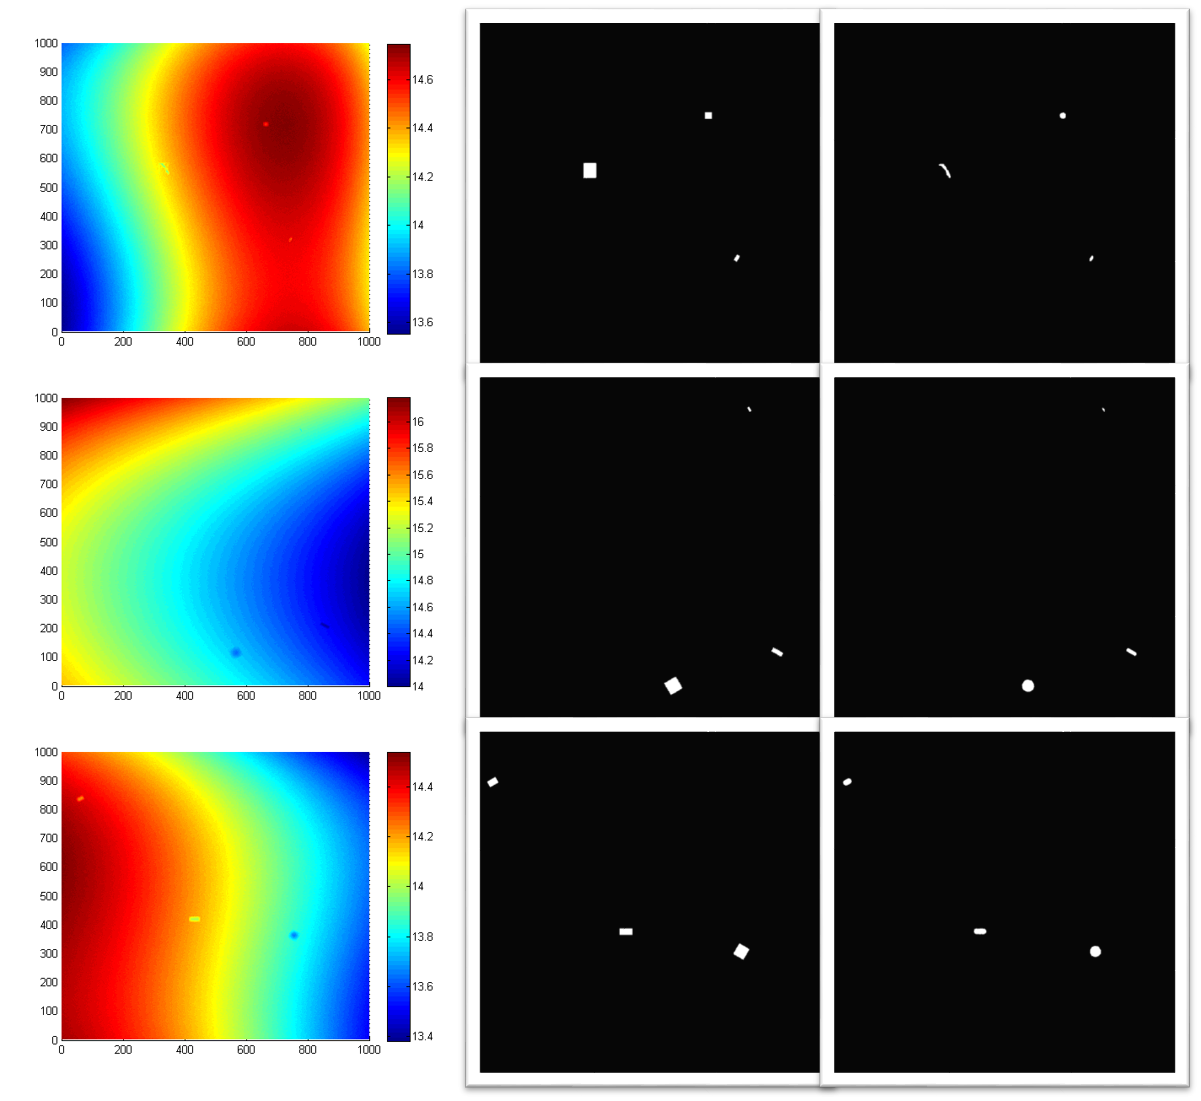
\includegraphics[width=16cm]{c4_plane_result.png}
        \caption{基于基准面拟合方法的部分实验结果}
        \label{fig:c4_plane_result}
        \end{figure*}

    \section{本章小结}
    \esection{Brief Summary}
    在本章中,我们提出了一种基于基准面拟合的深度图像缺陷检测算法。基于基准面的缺陷检测方法尝试去寻找钢板的基准面,然后将与基准面深度差别较大的区域作为缺陷种子点提取出来,最后使用基于种子点的图割方法来提取出完整的缺陷区域。

    另外,为了验证本文提出的两个缺陷检测算法,根据真实的钢板深度图像,我们使用人工合成的手段生成了一个钢板深度图像数据集,实验的结果显示,我们的方法达到了很好的效果。


        % multiple1902 <multiple1902@gmail.com>
% intro.tex
% Copyright 2011~2012, multiple1902 (Weisi Dai)
% https://code.google.com/p/xjtuthesis/
%
% It is strongly recommended that you read documentations located at
%   http://code.google.com/p/xjtuthesis/wiki/Landing?tm=6
% in advance of your compilation if you have not read them before.
%
% This work may be distributed and/or modified under the
% conditions of the LaTeX Project Public License, either version 1.3
% of this license or (at your option) any later version.
% The latest version of this license is in
%   http://www.latex-project.org/lppl.txt
% and version 1.3 or later is part of all distributions of LaTeX
% version 2005/12/01 or later.
%
% This work has the LPPL maintenance status `maintained'.
%
% The Current Maintainer of this work is Weisi Dai.
%

\chapter{基于法向量的缺陷检测算法}
\echapter{Normal Vector based Defect Detection Method}
由于基于基准面拟合的方法查准率较低,本章提出了基于法向量的缺陷检测算法,基于深度图像的法向量来检测缺陷区域,主要思路是利用法向量的余弦相似度来描述法向量的变化,根据输入的原始深度图像计算每个像素点的法向量,然后计算每个像素点与其邻域的法向量变化度量获得一张法向量梯度图像,接着根据法向量梯度图像使用双阈值分割获得候选的缺陷区域,最后验证候选区域的深度偏差是否达到了缺陷的定义,将满足缺陷定义的候选区域保留下来作为最终结果。
    \section{方法概述}
    \esection{Outline}
    钢板图像的缺陷区域往往在深度图像上表现为深度值上突然地落差,体现在法向量上能够理解为法向量的方向剧烈地变化。本算法根据法向量的余弦相似度来描述法向量之间的变化程度,对每一个像素点都计算其与邻域的法向量变化度量从而获得一张法向量梯度图像。法向量梯度图像直观的反映了深度值的平滑程度,法向量梯度值越大的地方越有可能是缺陷区域。

    该方法首先需要根据深度图像计算法向量,法向量一般被应用于点云数据的处理,深度图像本质上可以理解为结构化的点云数据。相对于在杂乱的点云上计算法向量,在深度图像上计算法向量要相对简单一些。Holzer等\cite{Holzer2012Adaptive}提出了两种利用积分图在深度图像上计算法向量的方法,第一种是根据水平向量和垂直向量的叉积来计算法向量,第二种是利用协方差矩阵来计算法向量。第一种法向量计算方法根据图像深度的变换求出对应点的水平向量和垂直向量,然后求出水平向量和垂直向量的叉积就得到法向量。第二种法向量计算方法利用协方差矩阵来计算法向量,根据对应点的领域信息,先计算它们的相应的协方差矩阵,然后计算这个协方差矩阵的特征向量,对应于最小特征值的特征向量就是计算得到的法向量,相较于利用叉积求法向量的方法,该方法虽然更加复杂和费时,但是利用协方差矩阵求法向量的方法更加准确可靠,并且协方差的特征向量能够直接体现对应点的领域平面的平面特性。我们主要使用基于协方差矩阵的方法来计算法向量,这种方法计算出的法向量更为平滑可靠。计算得到每个像素点的法向量之后,根据余弦相似度来计算法向量梯度图像,法向量梯度图像概念上类似于灰度图像的梯度图,主要用来检测法向量的变化情况。接着,使用双阈值分割来对法向量梯度图像进行二值化获得缺陷候选区域,最后对每个缺陷候选区域进行深度验证,检测其深度偏差是否达到缺陷的定义,最后把满足缺陷的深度定义条件的缺陷候选项输出作为最终的结果。

    基于法向量的缺陷检测算法流程如图\ref{fig:c5_flow_chart}所示,包括了计算法向量梯度图像,双阈值分割以及深度验证。

    \begin{figure*}[!h]
    \centering
    
\includegraphics[width=16cm]{c5_flow_chart.png}
    \caption{基于法向量的缺陷检测算法流程图}
    \label{fig:c5_flow_chart}
    \end{figure*}

    \section{计算法向量梯度图}
    \esection{Gradient Map of Normal Vector}
    法向量是指垂直于某一个平面的向量,对于一副深度图像而言,每个像素点跟其邻域的像素点能够拟合出一个局部的平面,该平面的法向量就是这个像素点的法向量,法向量的方向能够很好的表示出深度图像上的深度变化。

    法向量一般被应用于点云数据的处理,深度图像本质上可以理解为结构化的点云数据。相对于在杂乱的点云上计算法向量,在深度图像上计算法向量要相对简单一些。Holzer等\cite{Holzer2012Adaptive}提出了两种利用积分图来计算法向量的方法,第一种是根据水平向量和垂直向量的叉积来计算法向量,第二种是利用协方差矩阵来计算法向量。我们主要使用基于协方差矩阵的方法来计算法向量,这种方法计算出的法向量更为平滑可靠。

    在文章\cite{Holzer2012Adaptive}中,作者提出了两种法向量计算方法,并且采用了自适应的策略来确定计算法向量时领域半径的参数。第一种法向量计算方法根据图像深度的变换求出对应点的水平向量和垂直向量,然后求出水平向量和垂直向量的叉积就得到法向量。其原理如图\ref{fig:c5_normal_vector}所示。

    \begin{figure*}[!h]
    \centering
    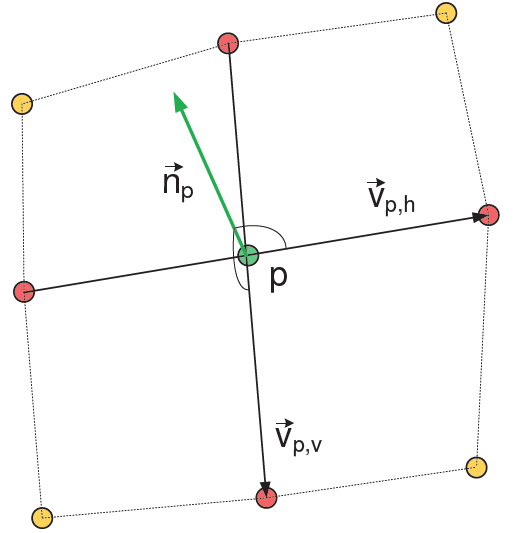
\includegraphics[width=8cm]{c5_normal_vector.png}
    \caption{法向量计算原理}
    \label{fig:c5_normal_vector}
    \end{figure*}

    第二种法向量计算方法利用协方差矩阵来计算法向量,根据对应点的领域信息,先计算它们的相应的协方差矩阵,然后计算这个协方差矩阵的特征向量,对应于最小特征值的特征向量就是计算得到的法向量,相较于利用叉积求法向量的方法,该方法虽然更加复杂和费时,但是利用协方差矩阵求法向量的方法更加准确可靠,并且协方差的特征向量能够直接体现对应点的领域平面的平面特性。

    计算得到每个像素点的法向量之后,根据余弦相似度来计算法向量梯度图像,法向量梯度图像概念上类似于灰度图像的梯度图,主要用来检测法向量的变化情况。假定$N\left({r,c}\right)$代表了点$\left({r,c}\right)$的法向量,那么点$\left({r,c}\right)$的法向量梯度值$g_n\left({r,c}\right)$表示为:
    \begin{eqnarray}
    g_n\left({r,c}\right)=\sqrt{{g_h\left({r,c}\right)}^{2}+{g_v\left({r,c}\right)}^{2}}
    \end{eqnarray}
    其中$g_h\left({r,c}\right)$和$g_v\left({r,c}\right)$分别表示为点$\left({r,c}\right)$ 在水平方向和垂直方向上的梯度值。$g_h\left({r,c}\right)$和$g_v\left({r,c}\right)$的公式表达为:
    \begin{eqnarray}
    g_h\left({r,c}\right)=C\left({N\left({r,c}\right),N\left({r,c-1}\right)}\right)+C\left({N\left({r,c}\right),N\left({r,c+1}\right)}\right)
    \end{eqnarray}
    \begin{eqnarray}
    g_v\left({r,c}\right)=C\left({N\left({r,c}\right),N\left({r-1,c}\right)}\right)+C\left({N\left({r,c}\right),N\left({r+1,c}\right)}\right)
    \end{eqnarray}
    公式中函数$C$表示计算计算两个法向量之间的相似性度量,函数$C$的公式为:
    \begin{eqnarray}
    C\left({n_1,n_2}\right)=1-abs\left({\frac{dot\left({n_1,n_2}\right)}{{\left\|n_1\right\|}_2*{\left\|n_2\right\|}_2}}\right)
    \end{eqnarray}
    其中$abs$函数为求绝对值函数,$dot$函数表示求两个向量的点积,${\left\|n\right\|}_2$ 定义为向量$n$的二范数。

    在扫描完整张图像,对每个像素点都计算得到其法向量梯度值之后,我们就得到了一张法向量梯度图像。法向量梯度图像非常类似于灰度图像的梯度图,不同的是法向量梯度图像表示一个邻域内法向量方向的变化,而灰度图像的梯度图表示灰度值的变化。

    法向量梯度图像的效果如图\ref{fig:c5_gradient}所示,从左至右依次为深度图像三维伪彩图、法向量梯度图像。

    \begin{figure*}[!h]
    \centering
    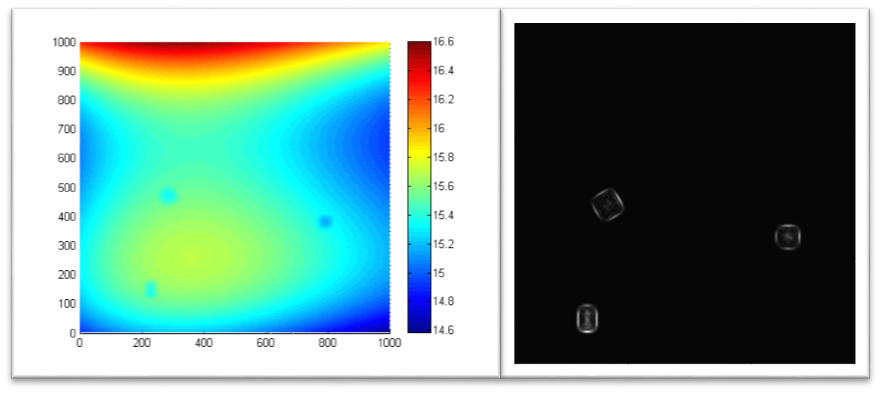
\includegraphics[width=16cm]{c5_gradient.png}
    \caption{法向量梯度图像}
    \label{fig:c5_gradient}
    \end{figure*}

    \section{双阈值分割}
    \esection{Dual Threshold Segmentation}
    在钢板缺陷检测领域,双阈值分割使用地非常频繁,这种类似于canny边缘算子\cite{Canny1986A} 的高低阈值设置方式在工程上被认为是简单可行并切实有效的。

    对法向量梯度图像使用高低阈值分别分割之后,获得了两张二值图像。双阈值分割的公式一般表达为:
    \begin{eqnarray}
    \left\{ \begin{array}{l}
    {B_{high}}\left( {r,c} \right) = 1,{g_n}\left( {r,c} \right) > {T_{high}}\\
    {B_{high}}\left( {r,c} \right) = 0,otherwise
    \end{array} \right.
    \end{eqnarray}
    \begin{eqnarray}
    \left\{ \begin{array}{l}
    {B_{low}}\left( {r,c} \right) = 1,{g_n}\left( {r,c} \right) > {T_{low}}\\
    {B_{low}}\left( {r,c} \right) = 0,otherwise
    \end{array} \right.
    \end{eqnarray}
    分割后的二值图像描述了缺陷区域的边缘信息,然而我们更关心的是缺陷部分的连通区域。所以我们首先使用3x3的正方形形态学算子对低阈值二值图像进行膨胀操作将一些断裂的边缘重新连接起来,接着对膨胀后的二值图像使用孔洞填充算法填充边缘二值图像的内部区域。接着对二值图像使用二值标记算法来获取候选缺陷连通区域获得两张连通区域标记图像${L_{low}}\left( n \right)$和${L_{high}}\left( m \right)$($n$和$m$表示连通区域的标记索引,$n = 1, \ldots ,N$,$m = 1, \ldots ,M$)。对低阈值连通区域标记图像$L_{low}$中的任一连通区域,如果它包含了高阈值连通区域标记图像$L_{high}$的连通区域,就将它保留,否则,舍弃。这个过程公式为:
    \begin{eqnarray}
    \left\{ \begin{array}{l}
    {B_{double}}\left( {{L_{low}}\left( n \right)} \right) = 1,{L_{high}}\left( m \right) \subset {L_{low}}\left( n \right)\\
    {B_{double}}\left( {{L_{low}}\left( n \right)} \right) = 0,otherwise
    \end{array} \right.
    \end{eqnarray}
    假定$L\left(i\right)$表示连通区域标记图像$L$中索引为$i$的连通区域的点集。经过双阈值分割后,最终分割出来的二值图像$B_{double}$中的连通区域就是候选的缺陷区域。在双阈值分割过程中,高低阈值$T_{high}$和$T_{low}$的选择比较重要,高阈值$T_{high}$的设置需要使得分割出来的二值图像查准率尽可能高,而低阈值$T_{low}$的设置需要使得查全率尽可能高。

    双阈值分割的结果如图\ref{fig:c5_double_thresh}所示,从左至右依次为法向量梯度图像、高阈值分割二值图、低阈值分割二值图、最终结果。

    \begin{figure*}[!h]
    \centering
    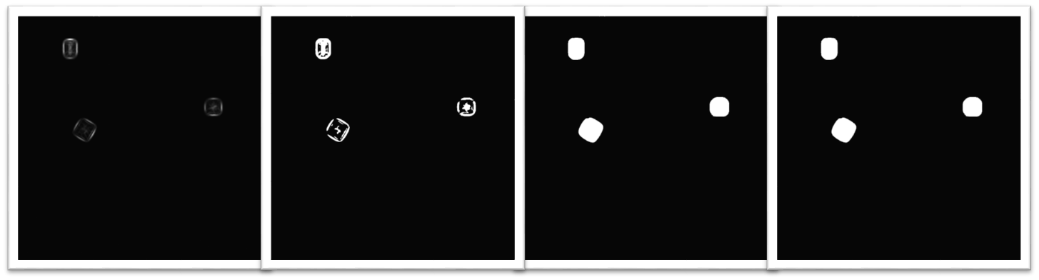
\includegraphics[width=16cm]{c5_double_thresh.png}
    \caption{双阈值分割实验结果}
    \label{fig:c5_double_thresh}
    \end{figure*}

    \section{深度验证}
    \esection{Verification of Depth}
    法向量梯度图像表示了像素点法向量变化的显著程度,所以在法向量梯度图像上分割后获得的连通区域在其边缘上法向量改变较明显。这一特点符合缺陷的特征,然而并不充分,因为根据定义缺陷不仅在其边缘上法向量存在剧烈的变化,其深度相对于正常钢板平面也存在较大的差异,所以对于每个候选的缺陷区域,都需要进行深度值的验证。

    对于一个候选的缺陷区域,首先对其矩形包围盒进行扩大,保持矩形包围盒的中心不变,将其长宽都扩大为之前的3倍,这样做是为了获得候选缺陷区域周边的局部上下文信息。接着对扩大后的局部深度图像使用章节4.2中的基准面拟合方法拟合出基准面,然后根据局部深度图像和基准面计算连通区域内每个像素点的深度偏差的最大值,若该最大值大于某个阈值,则保留该连通区域作为缺陷区域。这一过程用公式表达为:
    \begin{eqnarray}
    \left\{ \begin{array}{l}
    Label\left( i \right) = 1,\mathop {\max }\limits_{k \in P\left( i \right)} \left( {{d_{norm}}\left( k \right) - f\left( k \right)} \right) > {T_{depth}}\\
    Label\left( i \right) = 0,otherwise
    \end{array} \right.
    \end{eqnarray}
    其中$label\left(i\right)$表示对索引为$i$的连通区域的标记,其值为1代表作为缺陷保留,为0代表舍弃,$P\left(i\right)$代表该连通区域的点集。$k$代表一个像素点,$d_{norm}\left(k\right)$和$f\left(k\right)$分别代表该像素点在基准面的深度值和原始深度图像的深度值。

    \section{实验结果}
    \esection{Experimental Results}
        \subsection{数据集与评价方法}
        \esubsection{Data-set and Evaluation Protocol}
        本章的方法使用章节4.5.1提出的人工合成钢板深度图像数据集来检测算法的效果。同样的,对于检测算法检出的一个缺陷连通区域,我们使用连通区域包围盒的重叠率来判断检测是否成功,假定$R_p$为检测算法检测出的缺陷连通区域包围盒,$R_t$是已标记的缺陷连通区域包围盒,若$\frac{{R_p}\bigcap{R_t}}{{R_p}\bigcup{R_t}}>T_{overlap}$,即包围盒重叠率大于某个阈值则认为检测算法检出的该连通区域是一个缺陷。我们使用查全率、查准率和F值来评价算法的最终检测效果。
        \subsection{实验结果与分析}
        \esubsection{Experimental Results and Analysis}
        我们使用Matlab语言实现了本文提出的两个深度图像缺陷检测算法,实验用的计算机配置为:Intel Xeon E3-1241 3.50GHz CPU、32GB内存、Windows 7操作系统。处理一张1000x1000的深度图像,基于法向量的方法平均处理时间为60s。

        基于协方差矩阵来计算法向量,根据对应点的领域信息,先计算它们的相应的协方差矩阵,然后计算这个协方差矩阵的特征向量,对应于最小特征值的特征向量就是计算得到的法向量。使用MATLAB实现的部分代码如下所示,这部分代码实现了利用协方差矩阵来求解法向量。

        \lstinputlisting{code/get_normal_vector2.m}

        计算得到每个像素点的法向量之后,根据余弦相似度来计算法向量的梯度图像,法向量梯度图像在概念上类似于灰度图像的梯度图,主要用来检测法向量的变化情况。下面这部分代码实现了根据每个点的法向量来计算法向量梯度图像。

        \lstinputlisting{code/get_gradient_from_normal_vector.m}

        基于法向量的方法利用了缺陷部分的法向量变化较为剧烈这一特征,使用法向量梯度图像来刻画法向量的变化程度,概念上类似于灰度图像的梯度图,接着使用双阈值分割来获得候选缺陷区域,最终使用深度验证来确定候选缺陷区域是否为真正的缺陷。下面这部分代码表示了基于法向量方法检测缺陷的基本流程。

        \lstinputlisting{code/normal_detect_defect.m}

        本章中提出的基于法向量的深度图像缺陷检测算法在人工合成深度图像数据集上进行了实验,并评估了实验结果,实验结果如表\ref{tbl:c5_nvector_result}所示:

        \begin{table*}[!h]
        \centering
        \caption{基于法向量方法的实验结果}
        \label{tbl:c5_nvector_result}
        \begin{tabularx}{\columnwidth}{>{\centering\arraybackslash}X >{\centering\arraybackslash}X >{\centering\arraybackslash}X >{\centering\arraybackslash}X}
        \toprule
        方法 & 查全率 & 查准率 & F值 \\
        \midrule
        基于法向量 & 0.872 & 0.99 & 0.927 \\
        \bottomrule
        \end{tabularx}
        \end{table*}

        对于基于法向量的方法,输入可以是结构化点云数据,也可以是深度图像。由于深度图像只给出的每个像素点世界坐标系下的z轴坐标,没有x坐标和y坐标的信息,所以我们使用深度图像的像素坐标系的x坐标和y坐标来代替世界坐标系下的x坐标和y坐标。因为像素坐标系与世界坐标系之间可以通过单应性矩阵相互转换,这样做实际上并不会影响最终的实验效果,但是双阈值分割时阈值的设定会不一样。我们在实验中输入深度图像,使用协方差矩阵方法计算法向量时窗口半径设置为5,双阈值分割时高阈值$T_{high}$设置为$1*{10}^{-6}$,低阈值$T_{low}$ 设置为$T_{high}*0.1$,跟基于基准面的缺陷检测算法相同,深度验证时$T_{depth}$设置为0.1mm。

        本章提出的基于法向量的深度图像缺陷检测算法在人工合成的数据集上都达到了令人满意的效果。基于法向量的方法查准率较高,误检的情况较少,但是其查全率较低,存在缺陷未能检出的情况,主要原因可能是双阈值分割时阈值的设定较为苛刻。

        相比较与基于基准面拟合的缺陷检测算法,基于法向量的缺陷检测算法查准率较高,但是查全率相对较低,分析实验结果,基于法向量的缺陷检测算法容易漏检一些较小的缺陷,主要是因为较小的缺陷其法向量的变化程度相对不明显,所以反应在法向量的梯度图像上其梯度值较低,另外基于法向量的缺陷检测算法中,由于我们采用的是固定阈值,双阈值分割的高低阈值选择都需要足够的实验来确定,若想要提高查全率,可以尝试降低分割阈值,而这样做可能导致误检,降低查准率,所以基于法向量的方法阈值的确定较为困难。

        基于基准面拟合的方法往往能够分割出完整的缺陷轮廓,因为其最后一步采用了SFM水平集图像分割算法,而基于法向量的方法,由于其采用了形态学操作对分割后的二值图像进行了处理来将可能断裂的缺陷区域连接起来,其最终检出的缺陷轮廓并不完全准确,在实际应用中,缺陷轮廓并不准确影响并不大,钢厂一般更关心缺陷是否成功检出以及缺陷的位置,然而在实验评价中,基于法向量的方法处于劣势,可能有些缺陷区域基于法向量的方法实际上已经检出,但是由于检出的连通区域相对于groundtruth过大或者过小,导致被评价方法认定为没有检出。

        在人工合成数据集上的部分实验结果如图\ref{fig:c5_nvector_result}所示,从左至右依次为深度图像三维伪彩图、标记的缺陷区域、基于法向量算法的检测结果。

        \begin{figure*}[!h]
        \centering
        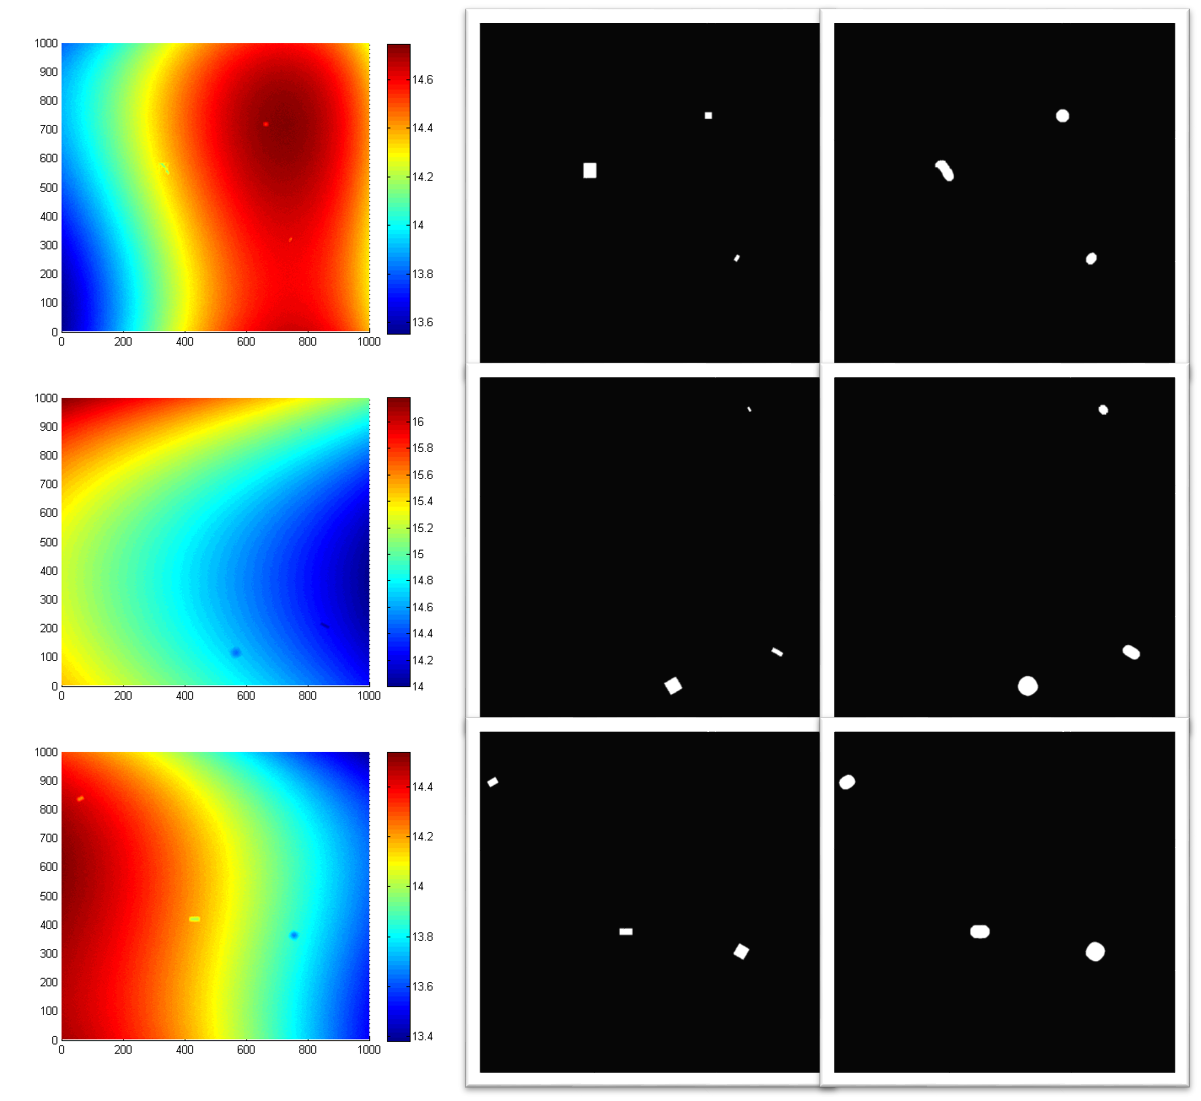
\includegraphics[width=16cm]{c5_nvector_result.png}
        \caption{基于法向量方法的部分实验结果}
        \label{fig:c5_nvector_result}
        \end{figure*}

    \section{本章小结}
    \esection{Brief Summary}
    在本章中,我们提出了一种基于法向量的深度图像缺陷检测算法。基于法向量的方法利用了缺陷部分的法向量变化较为剧烈这一特征,使用法向量梯度图像来刻画法向量的变化程度,概念上类似于灰度图像的梯度图,接着使用双阈值分割来获得候选缺陷区域,最终使用深度验证来确定候选缺陷区域是否为真正的缺陷。


        % multiple1902 <multiple1902@gmail.com>
% conclusion.tex
% Copyright 2011~2012, multiple1902 (Weisi Dai)
% https://code.google.com/p/xjtuthesis/
%
% It is strongly recommended that you read documentations located at
%   http://code.google.com/p/xjtuthesis/wiki/Landing?tm=6
% in advance of your compilation if you have not read them before.
%
% This work may be distributed and/or modified under the
% conditions of the LaTeX Project Public License, either version 1.3
% of this license or (at your option) any later version.
% The latest version of this license is in
%   http://www.latex-project.org/lppl.txt
% and version 1.3 or later is part of all distributions of LaTeX
% version 2005/12/01 or later.
%
% This work has the LPPL maintenance status `maintained'.
%
% The Current Maintainer of this work is Weisi Dai.
%
\chapter{结论与展望}
\echapter{Conclusions and Future Work}
    \section{结论}
    \esection{Conclusions}
    连铸坯在高速、自动化的连续生产过程中,由于受原材料、轨制设备、系统控制等诸多技术因素的影响,导致连铸坯表面出现划伤、压痕、裂纹、结疤、刮伤等不同类型的缺陷。这些缺陷将会严重影响连铸坯的质量,使得连铸坯的抗腐蚀性、抗疲劳性、耐磨性等性能大大降低。这就要求连铸坯生产企业要对连铸坯进行充分的缺陷检测,保障连铸坯的质量,以减少在生产过程中可能发生的各类严重事故。因此,连铸坯表面的缺陷检测就成为连铸坯生产过程中极其重要的环节。本文的主要工作有:

    1)对现有的连铸坯表面缺陷检测方法进行了整理和总结,现有的连铸坯表面缺陷检测方法主要分为传统无损方法、基于RGB图像的方法和基于深度图像的方法。传统无损方法其主要使用一些钢板的物理特性,通过钢板对电、热、磁等反应的变化来探测缺陷,这些方法往往存在一些局限性,并且方法的实时性不高。基于RGB图像的方法是目前连铸坯表面缺陷检测的研究热点,这些方法主要是使用CCD相机采集钢板灰度图像,然后使用一些图像处理的手段来检测缺陷位置,然而这些算法对于伪缺陷的误检率较高。基于深度图像的方法主要是使用钢板的深度图像来检测缺陷,利用深度信息能够有效地检测出缺陷并排除伪缺陷。

    2)提出了一种基于显著性的缺陷检测方法,很好地解决了目前基于机器视觉的低对比度带黑斑缺陷检测难点,通过该方法,检测出的缺陷更加完整,误检数量明显减少,由于结合了改进的显著性检测方法,去除了图像中黑斑伪缺陷对检测结果的干扰,同时,该方法检测速度快,完全符合缺陷检测中对时间性能的要求。当然,该方法仍有继续研究和改进的空间,如何更加完整的提取到缺陷区域、更加完全的去除黑斑,以及时间性能的进一步提高都将成为接下来的工作重点。

    3)提出了一种基于基准面拟合的钢板深度图像缺陷检测算法。基于基准面的缺陷检测方法尝试去寻找钢板的基准面,然后将与基准面深度差别较大的区域作为缺陷种子点提取出来,最后使用基于种子点的图割方法来提取出完整的缺陷区域。另外,为了验证本文提出的两个缺陷检测算法,根据真实的钢板深度图像,我们使用人工合成的手段生成了一个钢板深度图像数据集,实验的结果显示,我们的方法达到了很好的效果。

    4)提出了一种基于法向量的深度图像缺陷检测算法。基于法向量的方法利用了缺陷部分的法向量变化较为剧烈这一特征,使用法向量梯度图像来刻画法向量的变化程度,概念上类似于灰度图像的梯度图,接着使用双阈值分割来获得候选缺陷区域,最终使用深度验证来确定候选缺陷区域是否为真正的缺陷。
    \section{展望}
    \esection{Future Work}
    本文一共提出了三种连铸坯钢板表面缺陷检测算法,其中,基于显著性图的缺陷检测算法是基于RGB图像的方法,基于基准面拟合的方法和基于法向量的方法是基于深度图像的方法。总结一下目前方法的不足之处,未来的工作主要集中在一下几点:

    1)对于基于显著性的方法,如何减少伪缺陷的误检率是关键,我们设计了一个流程来去除图像中的黑斑,但是对于钢板图像来说,伪缺陷除了黑斑还有氧化铁皮、水膜等等,如何改进算法使之对所有类型的伪缺陷都不产生误检同时对真正缺陷的检出率保持较高水平是未来的主要工作;

    2)需要收集连铸坯表面深度图像制作深度图像数据库,由于目前收集下载不到真实的连铸坯表面深度图像数据集,我们采用人工合成的手段制作了一个深度图像数据库,虽然在制作过程中我们尽可能地去拟合真实的钢板表面情况,但是在真正的连铸坯表面深度数据集上验证我们的算法的有效性还是有必要的;

    3)对于基于基准面拟合的方法,拟合出的基准面的质量直接决定了算法的缺陷检测性能,所以有必要对基准面拟合算法进一步研究和优化;

    4)对于基于法向量的方法,根据余弦相似度我们提出了一种法向量梯度图像来度量像素点之间法向量的差异,然而目前算法的查全率并不优秀,更改并设计一种新的度量方法来评价像素点之间法向量的差异是未来的主要研究内容。

    \xjtuendcontent

    % 将你要引用的文献的 BibTeX 放入 bibliography.bib
    \xjtubib{bibliography}

    \xjtuappendix
        % multiple1902 <multiple1902@gmail.com>
% appendice.tex
% Copyright 2011~2012, multiple1902 (Weisi Dai)
% https://code.google.com/p/xjtuthesis/
%
% It is strongly recommended that you read documentations located at
%   http://code.google.com/p/xjtuthesis/wiki/Landing?tm=6
% in advance of your compilation if you have not read them before.
%
% This work may be distributed and/or modified under the
% conditions of the LaTeX Project Public License, either version 1.3
% of this license or (at your option) any later version.
% The latest version of this license is in
%   http://www.latex-project.org/lppl.txt
% and version 1.3 or later is part of all distributions of LaTeX
% version 2005/12/01 or later.
%
% This work has the LPPL maintenance status `maintained'.
%
% The Current Maintainer of this work is Weisi Dai.
%

\iffalse
\xjtuappendixchapter{附录}
\xjtuappendixechapter{Appendices}
% 超过一个 section 时用 Appendices, 否则用 Appendix

    \xjtuappendixsection{二级标题}

        \xjtuappendixsubsection{三级标题}

            \xjtuappendixsubsubsection{四级标题}

    \xjtuappendixchapter{还是附录}

        \xjtuappendixsection{测试}
\fi

    \xjtuendappendix

    \xjtuspchapter{致谢}{致\qquad 谢}{Acknowledgements}
        % multiple1902 <multiple1902@gmail.com>
% acknowledgements.tex
% Copyright 2011~2012, multiple1902 (Weisi Dai)
% https://code.google.com/p/xjtuthesis/
%
% It is strongly recommended that you read documentations located at
%   http://code.google.com/p/xjtuthesis/wiki/Landing?tm=6
% in advance of your compilation if you have not read them before.
%
% This work may be distributed and/or modified under the
% conditions of the LaTeX Project Public License, either version 1.3
% of this license or (at your option) any later version.
% The latest version of this license is in
%   http://www.latex-project.org/lppl.txt
% and version 1.3 or later is part of all distributions of LaTeX
% version 2005/12/01 or later.
%
% This work has the LPPL maintenance status `maintained'.
%
% The Current Maintainer of this work is Weisi Dai.
%




    \xjtuspchapter{攻读硕士期间取得的研究成果}{攻读硕士期间取得的研究成果}{Achievements}
        % multiple1902 <multiple1902@gmail.com>
% acknowledgements.tex
% Copyright 2011~2012, multiple1902 (Weisi Dai)
% https://code.google.com/p/xjtuthesis/
%
% It is strongly recommended that you read documentations located at
%   http://code.google.com/p/xjtuthesis/wiki/Landing?tm=6
% in advance of your compilation if you have not read them before.
%
% This work may be distributed and/or modified under the
% conditions of the LaTeX Project Public License, either version 1.3
% of this license or (at your option) any later version.
% The latest version of this license is in
%   http://www.latex-project.org/lppl.txt
% and version 1.3 or later is part of all distributions of LaTeX
% version 2005/12/01 or later.
%
% This work has the LPPL maintenance status `maintained'.
%
% The Current Maintainer of this work is Weisi Dai.
%

\clearpage




    \xjtuacademicintegrity


\end{document}
